\documentclass[11pt]{article}

\usepackage[utf8]{inputenc}
\usepackage[margin=1in]{geometry}
\usepackage{amsmath,amssymb}
\usepackage{booktabs}
\usepackage{graphicx}
\usepackage{siunitx}
\usepackage{xcolor}
\usepackage{natbib}
\usepackage[hidelinks]{hyperref}
\usepackage{cleveref}

\graphicspath{{figures/}}

\title{\textbf{Benchmarking Out-of-Distribution Methods for Time Series:\\
A Fair, Faithful Evaluation on Streaming Distributional Shift}}
\author{Stylianos Giannoulis\\
Aristotle University of Thessaloniki\\
Department of Informatics\\
MSc in Data and Web Science\\
Supervisor: John Paparrizos}
\date{2026}

\begin{document}
\maketitle

\begin{abstract}
Detecting out-of-distribution (OOD) inputs is a prerequisite for the safe
deployment of machine-learning models on time series, where a confidently wrong
decision on an unseen regime can mask an industrial fault, a cardiac arrhythmia,
or a service outage. A large family of modality-agnostic OOD detectors has been
developed for vision and language, yet their reliability under \emph{streaming
distributional shift} --- the realistic setting in which a deployed model
gradually encounters a new source distribution --- remains under-explored. We
present a comprehensive, fair, and reproducible evaluation of seventeen OOD
detectors (of twenty-four audited candidates) on the two target families of the
TSB-StreamingAD benchmark, TSB-StreamingAD-U (univariate) and TSB-StreamingAD-M
(multivariate), in which each recording concatenates two source signals and OOD
is defined at the window level under a leakage-free source-boundary training
split. Across \num{527} datasets (\num{260} univariate and \num{267}
multivariate) and \num{8668} completed runs at seed \num{42}, distance- and
density-based detectors that model the in-distribution feature manifold dominate
post-hoc softmax and logit detectors: Mahalanobis distance (mean AUROC
\num{0.826}) and DFM-PCA (\num{0.812}) lead, whereas every post-hoc softmax,
logit, and gradient detector --- including maximum-softmax-probability
(\num{0.370}) and gradient-norm (\num{0.294}) --- together with the seasonal SRS
(\num{0.352}) falls below chance, several with \emph{inverted} scores. A Friedman
test confirms the ranking is highly significant ($\chi^2 = \num{2336.59}$, $p <
\num{1e-16}$). We trace the failure of output-head scores to an overconfidence
mechanism amplified by global normalisation, and we show that the winning
detectors are also Pareto-optimal in the accuracy--efficiency plane (top accuracy
at roughly \SIrange{1}{4}{\milli\second} per window). A faithfulness audit against
the original papers and official code reveals pervasive implementation drift in
the post-hoc detectors, yet even paper-faithful corrected variants do \emph{not}
become competitive --- the feature-space ranking is unchanged. We further report a
cautionary negative result: the correct orientation of energy-based scores is
regime-dependent, so a correction validated on synthetic data can reverse on real
data. Our findings corroborate and extend to the streaming setting the
recommendation that deep feature modeling is the most promising direction for
time-series OOD detection.
\end{abstract}

\section{Introduction}\label{sec:intro}

A sudden mechanical failure in a manufacturing plant produces sensor readings that
no training set anticipated; a patient's electrocardiogram drifts into an
arrhythmia morphology absent from the monitored history; a web service migrates to
infrastructure whose load profile the deployed anomaly detector has never seen. In
each case the model must do more than classify --- it must recognise that the
input lies outside the distribution it was trained on and abstain from a confident
answer. This is the task of out-of-distribution (OOD) detection, and on time
series it carries unusually high stakes because the data are continuous, temporally
dependent, and arrive as never-ending streams in which the underlying distribution
is free to change. A detector that silently fails on the first window of a new
regime defeats the very purpose of monitoring.

The state of the art in OOD detection has been shaped largely by computer vision.
Post-hoc scores that read a trained classifier --- the maximum softmax probability,
temperature-scaled logits, rectified or sparsified activations, gradient norms ---
are attractive because they require no retraining and no auxiliary data. The
reference study for this thesis, TS-OOD \citep{Gungor2025}, transplanted eight such
detectors to thirteen multivariate time-series datasets under a same-dataset
semantic-shift protocol and reached two conclusions: most vision-derived detectors
perform poorly on time series, and methods based on \emph{deep feature modeling} ---
Mahalanobis distance \citep{Lee2018} and feature reconstruction \citep{Ahuja2019}
--- are markedly more effective. What TS-OOD did not establish is whether these
conclusions survive a \emph{streaming} shift, in which the OOD signal is a transition
between two concatenated source recordings rather than a held-out class, and whether
they generalise beyond the eight original detectors to the broader landscape of
time-series-specific, drift, changepoint, and reconstruction methods that have since
appeared.

We close that gap with what is, to our knowledge, the most comprehensive fair
evaluation of OOD detectors on streaming time series to date. We evaluate
seventeen detectors --- spanning post-hoc softmax/logit, feature distance/density,
reconstruction, contrastive/self-supervised, drift/changepoint, and
time-series-specific families --- on the two target benchmark families
TSB-StreamingAD-U and TSB-StreamingAD-M, comprising \num{527} datasets and
\num{8668} completed runs. Crucially, we precede the evaluation with a
method-by-method audit of every implementation against its source paper and, where
available, its official code. All twenty-four are legitimate OOD methods from the
literature; seventeen are evaluated under a single unified streaming protocol, while
the remaining seven require adapted, method-appropriate protocols
(auxiliary-outlier training, ordered streams, a retrained feature extractor, or
batch-level scoring) and are evaluated and reported separately for fairness. Our
contributions are:

\begin{enumerate}
  \item \textbf{A streaming benchmark of seventeen detectors.} We evaluate every
  detector that passes the faithfulness gate on TSB-StreamingAD-U and
  TSB-StreamingAD-M under a single, leakage-free source-boundary protocol,
  reporting AUROC, AUPR, FPR@95, detection accuracy, and inference cost
  (\cref{sec:results}). Distance- and density-based detectors dominate: Mahalanobis
  distance (\num{0.826}) and DFM-PCA (\num{0.812}) attain the highest mean AUROC,
  while every post-hoc softmax, logit, and gradient detector falls below the
  \num{0.5} chance line, several with inverted scores.
  \item \textbf{A faithfulness audit as a first-class result.} We audit all
  twenty-four candidate implementations against their published descriptions and,
  where available, their official code (\cref{sec:setup,app:fidelity}); all
  twenty-four are legitimate OOD methods, seventeen evaluated under the unified
  streaming protocol and the remaining seven under adapted, method-appropriate
  protocols reported separately for fairness (\cref{sec:results-classd}). Several
  variants required validated, paper-faithful corrections; even so, the corrected
  post-hoc detectors remain uncompetitive (\cref{sec:discussion}).
  \item \textbf{A mechanistic explanation, with the univariate--multivariate
  contrast.} We attribute the post-hoc failure to output-head overconfidence on
  far-out inputs, amplified by global normalisation, and we document a
  normalisation dichotomy in which feature methods peak under global normalisation
  while post-hoc methods invert under both schemes (\cref{sec:discussion}). We
  further show that the univariate family is modestly \emph{easier} than the
  multivariate family for the feature methods, and explain why.
  \item \textbf{A deployment recommendation and a negative result.} We identify
  Mahalanobis distance and DFM-PCA as Pareto-optimal --- simultaneously the most
  accurate and among the fastest --- and recommend them as defaults for streaming
  deployment. We additionally report that the principled orientation of
  energy-based scores is regime-dependent, a cautionary negative result that
  disciplines the correction methodology itself.
\end{enumerate}

The remainder of the manuscript proceeds as follows. \Cref{sec:related} organises
the detector landscape into analytic clusters and positions this work.
\Cref{sec:datasets} describes every dataset family used, with special emphasis on
the two target benchmark families. \Cref{sec:methods} formalises the task and
catalogues all twenty-four detectors by algorithmic family, including the
paper-faithful corrected and adapted variants, and explains the unified-versus-adapted
evaluation split.
\Cref{sec:setup} details the hardware, reproducibility, metrics, protocol, and the
verification gate. \Cref{sec:results} reports the results. \Cref{sec:discussion}
analyses which methods generalise, which fail, and why. \Cref{sec:conclusion}
concludes with recommendations and future work.

\section{Related Work}\label{sec:related}

We group OOD detectors analytically rather than enumerate them, positioning this
work against each cluster. A recurring theme of benchmark studies in this area is
that apparent advances do not always survive a fair, like-for-like comparison; our
evaluation is designed to test exactly that.

\paragraph{Post-hoc softmax and logit methods.}
These read a frozen, in-distribution-trained classifier and require no retraining.
The maximum softmax probability (MSP) \citep{Hendrycks2017} treats low confidence
as evidence of OOD; ODIN \citep{Liang2018} sharpens the softmax with temperature
scaling and input perturbation; the energy score \citep{Liu2020} replaces
confidence with the log-sum-exp of the logits. Their shared assumption is that the
output head is well calibrated on inputs far from the training manifold --- an
assumption that fails badly, as a deep ReLU network can be arbitrarily confident on
far-out inputs \citep{Hein2019, Nguyen2015}. We show this failure is precisely what
sinks the cluster on streaming shift.

\paragraph{Activation-shaping and gradient methods.}
A related family modifies the classifier's internal signals before scoring. ReAct
\citep{Sun2021} clips extreme activations; DICE \citep{Sun2022} sparsifies the
classifier weights to emphasise discriminative directions; SCALE \citep{Xu2024}
rescales penultimate activations; ASH \citep{Djurisic2023} prunes and rescales late
activations; GradNorm \citep{Huang2021} uses the $L_1$ norm of the gradient of the
Kullback--Leibler divergence to a uniform distribution. These transformations were
tuned on vision benchmarks and, as our audit reveals, are also the methods most
prone to implementation drift when ported to time series.

\paragraph{Feature distance and density methods.}
Rather than the output head, these model the in-distribution \emph{feature}
manifold. Mahalanobis distance \citep{Lee2018} fits class-conditional Gaussians
with a tied covariance; deep feature modeling (DFM) \citep{Ahuja2019} fits a
per-class principal-component model and scores the feature reconstruction error;
incremental DFM \citep{Rios2022} extends this to continual settings. TS-OOD
\citep{Gungor2025} identified this family as the most promising for time series.
Our results extend that finding to the streaming regime, explain it
mechanistically, and reveal that several detectors marketed under other names
reduce to feature-space distance or density in disguise.

\paragraph{Reconstruction-based methods.}
Reconstruction detectors flag inputs they cannot reproduce. Diffusion-based
imputation \citep{Xiao2023} and transformer reconstruction \citep{Tuli2022} learn
normal behaviour and treat large reconstruction error as anomalous. Their fidelity
hinges on the reconstruction being \emph{driven by the input}; a model that samples
from the learned normal distribution unconditionally measures nothing about the
specific test window, a defect we encounter in audit.

\paragraph{Contrastive, self-supervised, and augmented-training methods.}
Outlier Exposure \citep{Hendrycks2019} and its diversified variant \citep{Zhu2023}
train the classifier against an auxiliary outlier set to force uniform predictions
off-distribution; a provable diversification framework \citep{Diversification2024}
formalises when this helps. The defining mechanism is auxiliary-outlier training,
which the unified frozen-backbone streaming protocol cannot supply; we therefore
evaluate these three methods under adapted protocols (auxiliary-outlier fine-tuning
arms) reported in \cref{sec:results-classd}, where a faithful rebuild without an
auxiliary corpus reduces to an energy baseline.

\paragraph{Drift, changepoint, and time-series-specific methods.}
A distinct lineage exploits temporal structure directly. Seasonal-ratio scoring
\citep{Belkhouja2023} compares observed values to seasonality-aware expectations via
STL decomposition and conditional VAEs; conformal temporal non-conformity
\citep{Kaur2023} provides false-detection guarantees; InvAD \citep{InvAD2025}
uses invertible networks; M2N2 \citep{M2N22024} performs memory-based test-time
adaptation; DiMMAD \citep{DiMMAD2025} ensembles distance metrics; DEEDEE
\citep{DEEDEE2025} targets concept drift; and CatSight \citep{CatSight2023} applies
common-spatial-pattern analysis to multivariate streams. A further group requires
evaluation protocols the unified streaming setting cannot realise: DIVERSIFY
\citep{Lu2024} learns environment-invariant representations adversarially by
retraining the extractor; TD-IVDM \citep{TDIVDM2025} uses multi-scale ordered windows;
DriftLens \citep{Greco2025} tracks batch-level distributional change in deep
embeddings; and an autoencoder--ADWIN--LSTM hybrid \citep{AEADWINLSTM2025} needs an
ordered stream. We evaluate these four under adapted, method-appropriate protocols
(reported in \cref{sec:results-classd}). These methods are rarely compared head-to-head
under a single protocol; the benchmark and library efforts of \citet{Zhang2023},
\citet{VanLooveren2020}, and \citet{Montiel2021} aggregate implementations but not a
fair like-for-like comparison on streaming OOD. We provide exactly such a
comparison, and find that several of these ``time-series-specific'' detectors are,
under their per-sample implementations, generic feature-space estimators.

\paragraph{Position of this work.}
Our study sits in the empirical-benchmark lineage of \citet{LiuTSBAutoAD2025} and
\citet{Gungor2025}: confidence comes from breadth and statistical rigour, not from
proposing a new method. We extend \citet{Gungor2025} along three axes --- a
streaming distributional-shift regime in place of static semantic shift, a method
pool of twenty-four audited detectors in place of eight, and a verify-before-experiment gate
that treats implementation faithfulness as a measured quantity rather than an
assumption.

\section{Datasets}\label{sec:datasets}

We evaluate on the two target families of the TSB-StreamingAD benchmark and draw on
two auxiliary collections for verification and calibration only. We describe each in
turn, emphasising content, structure, anomaly characteristics, streaming
characteristics, expected difficulty, and why it is included.

\subsection{TSB-StreamingAD-U and TSB-StreamingAD-M}\label{sec:tsb}

The two target families, TSB-StreamingAD-U (univariate) and TSB-StreamingAD-M
(multivariate), are collections of long \emph{streaming} time-series files derived
from the TSB-StreamingAD anomaly-detection benchmark. Each file has one or more
numeric feature columns followed by a binary \texttt{Label} column (0 = normal, 1 =
anomalous). The full TSB-StreamingAD-U and TSB-StreamingAD-M families contain
\num{300} files each; the per-file statistics reported below are computed over all
\num{600} files, while the headline detector sweep covers \num{527} datasets
(\num{260} univariate and \num{267} multivariate) spanning the DRIFT/OOD/STABLE
categories.

\paragraph{Two-source construction.}
Each file is built by concatenating \emph{two source recordings}. Source~1 (S1) is a
normal recording; Source~2 (S2) introduces a distribution shift and is labelled
anomalous. The first anomalous timestep marks the S1/S2 boundary, so all S1
timesteps are normal by construction. The filename encodes the construction (e.g.\
\texttt{DRIFT\_003\_SEG\_..\_<SRC1>\_..\_AND\_<SRC2>\_..}). This single-shift-event
design is the defining streaming characteristic: rather than scattered point
anomalies, each series contains one regime transition, and the anomalous S2 region
is a contiguous tail.

\paragraph{Window-level OOD.}
A sliding window of fixed size and stride (default \numproduct{64 x 32}; configurations
also use \numproduct{128 x 64}) is swept over the series. A window is ID (label 0) if
\emph{all} its timesteps are normal, and OOD (label 1) if it contains \emph{any}
anomalous timestep. Normal S1 windows constitute the in-distribution data; OOD
windows come from the shifted S2 region.

\paragraph{Source-boundary split.}
The backbone is trained \emph{only} on S1 normal windows --- those ending strictly
before the boundary --- using \SI{70}{\percent} of that pool. Held-out S1 normals
form the ID evaluation windows and all anomalous windows form the OOD evaluation
windows; the evaluation pool is balanced 1:1 and split \SI{50}{\percent}/%
\SI{50}{\percent} into validation and test. This split forbids S2 signal from
leaking into training, which would otherwise collapse AUROC toward \num{0.5} by
letting the backbone memorise the shift.

\paragraph{Composition and structure.}
Both families are balanced across three categories: \num{100} DRIFT, \num{100} OOD,
and \num{100} STABLE files each. The families differ sharply in dimensionality and
scale. TSB-U is strictly univariate (one channel), with series length ranging from
\num{2842} to \num{1030400} timesteps (median \num{20060}) and median anomaly rate
\SI{0.53}{\percent}. TSB-M is multivariate, with channel counts from \num{2} to
\num{248} (median \num{19}), series length from \num{3399} to \num{880400} (median
\num{329198}), and median anomaly rate \SI{5.23}{\percent} --- roughly ten times
denser than TSB-U. The first-anomaly boundary sits at a median fraction of
\num{0.169} of the series in TSB-U and \num{0.181} in TSB-M, so the S1 training
region is typically the first fifth of each file. The two families also span
different application domains: TSB-U is dominated by WebService (\num{150} files) and
Medical (\num{74}) sources, whereas TSB-M is dominated by Medical (\num{135}) and
Facility (\num{116}) sources, with multivariate Sensor (\num{47}) recordings.

\paragraph{Categories and expected difficulty.}
The DRIFT/OOD/STABLE axis is a controlled difficulty axis. In DRIFT files, S2 is a
\emph{related but drifted} recording: the shift is subtle and S2 window
representations overlap substantially with S1, so detectors must separate
near-distribution drift (expected difficulty medium--high). In OOD files, S2 is a
\emph{clearly different} regime, so window features are more separable from the S1
manifold (expected difficulty low--medium; the easier, cleanly separable category).
STABLE files pair \emph{similar/stationary} sources with little genuine shift, acting
as negative/control cases: a well-calibrated detector should \emph{not} over-flag
them, so high-false-positive methods are penalised here (a specificity check).

\paragraph{Why these are the right target.}
These two families are the thesis target because they (i) provide labelled,
window-level OOD ground truth under a single reproducible protocol shared across all
detectors; (ii) span a controlled difficulty axis (STABLE specificity control,
subtle DRIFT, strong OOD), letting us measure not just average AUROC but \emph{where}
a method's separation power and calibration break down; and (iii) cover both
univariate and multivariate regimes across multiple domains, testing whether OOD
scores generalise across channel counts and modalities. The source-boundary split
makes the task honest by forbidding S2 leakage, so AUROC reflects true
generalisation rather than memorisation.

\subsection{Auxiliary collections}\label{sec:aux}

Two further collections are used only for verification and calibration, never for
headline claims. The \emph{UCR/UEA} multivariate archive \citep{Dau2019, Bagnall2018}
is the static semantic-shift benchmark of the reference study \citep{Gungor2025},
where the first half of the classes is treated as ID and the second half as OOD; we
reference it to anchor our protocol against prior work but do not re-evaluate it
here. A \emph{synthetic validation set} --- a controlled task of in-distribution and
out-of-distribution series with a known separating signal --- is used to verify that
each detector implementation produces a finite, correctly oriented score before it
enters the streaming sweep. The synthetic set deliberately does not stress the
streaming-specific failure modes, which is itself a finding we discuss in
\cref{sec:discussion}.

\section{Methods}\label{sec:methods}

We first formalise the task and metrics, then catalogue every audited detector by
algorithmic family. All twenty-four detectors are legitimate OOD methods from the
literature and are described here as first-class methods within their natural
family; for those whose audit produced a paper-faithful correction we describe both
the original and the corrected (\texttt{\_enh}) variant. The distinction relevant to
this study is not methodological but procedural. Seventeen detectors can be evaluated
under a single \emph{unified} fair-comparison streaming protocol --- a shared frozen
ResNet backbone, per-window shuffled evaluation, and no auxiliary outlier corpus ---
while the other seven \emph{require} an \emph{adapted} protocol: auxiliary-outlier
training, an ordered stream, a retrained feature extractor, or batch-level scoring.
The latter seven are therefore evaluated under those method-appropriate adapted
protocols and reported separately for fairness (\cref{sec:results-classd},
\cref{tab:class_d_appendix}); this is an evaluation constraint, not an exclusion, and
we flag each method's evaluation arm as we describe it.

\subsection{Problem formulation}\label{sec:problem}

Let a time series be $X = \{x_1, \dots, x_T\}$ with $x_t \in \mathbb{R}^{d}$. A
sliding window of length $w$ and stride $s$ yields windows $W_i \in \mathbb{R}^{d
\times w}$. Each recording concatenates two source signals; a window is
\emph{in-distribution} (ID) if all its timesteps belong to the first source and are
normal, and \emph{out-of-distribution} (OOD) if it contains any anomalous timestep.
We write $P_{\mathrm{in}}$ for the ID window distribution and $P_{\mathrm{out}}$ for
the OOD distribution. An OOD detector is a scoring function $s : \mathbb{R}^{d
\times w} \to \mathbb{R}$ for which larger values indicate greater anomalousness.

A backbone $f_\theta$ is trained only on ID windows, using cross-entropy over $K$
pseudo-classes formed by partitioning the ID training windows into $K$ equal temporal
bins. Detectors are fit on ID data only and never observe OOD data during training;
they are merely evaluated on it. We assume no OOD data is available at training time
and that the ID training pool is uncontaminated by the second source --- an
assumption enforced by the source-boundary split (\cref{sec:tsb}) and whose
violation we treat as a threat to validity.

\subsection{Metrics}\label{sec:metrics}

Given test scores $\{s_i\}$ and binary labels $\{y_i\}$ ($y_i = 1$ for OOD), we
report four threshold-aware and threshold-free metrics:
\begin{align}
\mathrm{AUROC} &= \Pr\big(s(X^{+}) > s(X^{-})\big), \quad X^{+}\!\sim P_{\mathrm{out}},\; X^{-}\!\sim P_{\mathrm{in}}, \\
\mathrm{AUPR}  &= \int_0^1 \mathrm{Prec}(r)\,\mathrm{d}r, \\
\mathrm{FPR@95} &= \mathrm{FPR}\big(\tau^{*}\big), \quad \tau^{*} : \mathrm{TPR}(\tau^{*}) = 0.95,
\end{align}
where AUROC and AUPR are threshold-free and $\tau^{*}$ is fixed on the validation
set. We additionally report detection accuracy at the validation-optimal threshold
and the per-sample inference time. AUROC is our primary metric because it is
threshold-independent and invariant to the 1:1 class balance of the evaluation pool;
an AUROC below \num{0.5} indicates a score that separates ID from OOD but with the
\emph{wrong} sign, a phenomenon central to our findings.

\subsection{Post-hoc softmax and logit detectors}\label{sec:m-posthoc}

\paragraph{Maximum Softmax Probability (MSP).}
MSP scores $s(X) = 1 - \max_c \mathrm{softmax}(f_\theta(X))_c$
\citep{Hendrycks2017}: low confidence is read as OOD. It assumes the head is
calibrated off-distribution. Cost is a single forward pass. We expect it to fail when
the head is overconfident on far-out windows.

\paragraph{ODIN.}
ODIN \citep{Liang2018} adds temperature scaling ($T=1000$) and an input perturbation
$x - \varepsilon\,\mathrm{sign}(\nabla_x \mathrm{CE})$ to sharpen ID/OOD separation,
then scores $1 - \max_c \mathrm{softmax}$. It inherits MSP's assumption and adds a
gradient computation, roughly multiplying cost by the perturbation steps.

\paragraph{Energy (EBO).}
The energy score \citep{Liu2020} replaces softmax confidence with the negative
log-sum-exp of the logits, $s(X) = -T\log\sum_c \exp(f_\theta(X)_c / T)$, a
temperature-free, training-free logit statistic. It is faithful as implemented and
enters the benchmark directly; it is also the clean baseline that the
auxiliary-outlier-training methods (Outlier Exposure, DivOE) reduce to when their
defining auxiliary training is unavailable under the unified protocol
(\cref{sec:m-augmented}). Cost is a single forward pass.

\paragraph{ReAct (original and \texttt{react\_enh}).}
ReAct \citep{Sun2021} clips activations at a global percentile ($p=90$) before
scoring. The original implementation computes MSP on the clipped logits; the
published headline configuration is ReAct~+~energy. \textbf{Implementation note.} We
identified and corrected an inconsistency between the implementation and the
procedure described in \citet{Sun2021}: the corrected variant computes the energy
score after activation clipping. We refer to it as \texttt{react\_enh}.

\paragraph{DICE (original and \texttt{dice\_enh}).}
DICE \citep{Sun2022} sparsifies the classifier weights by importance, then computes
energy on the sparsified logits. \textbf{Implementation note.} The original
implementation selected the top-$k$ entries of $\text{feature}\odot\text{weight}$
per sample, summed their \emph{absolute} values, and computed MSP; the corrected
\texttt{dice\_enh} sums the \emph{signed} top-$k$ contributions and computes energy,
matching \citet{Sun2022}.

\paragraph{SCALE (original and \texttt{scale\_enh}).}
SCALE \citep{Xu2024} rescales penultimate activations by a factor derived from the
top-$p$ percentile, then computes energy. \textbf{Implementation note.} The original
implementation z-standardised the \emph{logits} instead; the corrected
\texttt{scale\_enh} applies activation scaling at the penultimate layer per
\citet{Xu2024}.

\paragraph{GradNorm (original and \texttt{gradnorm\_enh}).}
GradNorm \citep{Huang2021} uses the $L_1$ norm of the gradient of the
KL-to-uniform loss with respect to the \emph{last-layer weights}; ID samples have
\emph{larger} gradient norm than OOD. \textbf{Implementation note.} The original
implementation backpropagated a cross-entropy-to-predicted-label loss to the
\emph{input}, took the $L_2$ norm, and inverted the orientation --- a different
statistic with the opposite sign. The corrected \texttt{gradnorm\_enh} computes the
$L_1$ norm of the last-layer-weight gradient of the KL-to-uniform objective and sets
the score to its negation, matching \citet{Huang2021}.

\subsection{Feature distance and density detectors}\label{sec:m-feature}

\paragraph{Mahalanobis distance (MDS).}
With class-conditional means $\mu_c$ and tied covariance $\Sigma$ on ID pre-logit
features, $s(X) = \min_c \sqrt{(\phi(X)-\mu_c)^\top \Sigma^{-1}(\phi(X)-\mu_c)}$
\citep{Lee2018}. Relative to the original we omit the FGSM perturbation and the
multi-layer ensemble exactly as \citet{Gungor2025} prescribe for multivariate time
series. \textbf{Implementation note.} The audited variant mis-estimated the tied
covariance; the corrected variant uses the within-class scatter (tied-covariance)
estimate of \citet{Lee2018}, and it is the corrected form that enters the benchmark.
It assumes ID features are approximately Gaussian; cost is one matrix solve per
window ($\sim$\SI{1}{\milli\second}). We expect it to lead.

\paragraph{DFM-PCA.}
A principal-component model is fit per ID class; $s(X) = \min_c \lVert \phi(X) -
\mathrm{PCA}_c^{-1}(\mathrm{PCA}_c(\phi(X))) \rVert$ \citep{Ahuja2019}. It models the
ID feature manifold and scores reconstruction error, assuming OOD features leave the
principal subspace. Cost is low. \citet{Gungor2025} identify this family as the most
promising for time series.

\paragraph{DiMMAD (\texttt{dimmad\_enh}).}
DiMMAD \citep{DiMMAD2025} ensembles distance metrics in feature space.
\textbf{Implementation note.} The original ensemble included binary/set metrics
(Hamming, Jaccard, Dice) applied to continuous deep features, where they are
ill-defined; the corrected \texttt{dimmad\_enh} restricts the ensemble to continuous
metrics (Euclidean, Manhattan, Mahalanobis, cosine, correlation, Canberra,
Bray--Curtis). It is reported only in its corrected form.

\subsection{Augmented-training detectors}\label{sec:m-augmented}
These methods sharpen OOD separation by training the classifier against an auxiliary
outlier set so that it emits (near-)uniform predictions off-distribution. Their
defining mechanism is auxiliary-outlier training, which the unified frozen-backbone
protocol cannot supply; we therefore evaluate all three under an adapted protocol ---
head-only or full-network fine-tuning arms with a synthesised or held-out outlier
corpus --- reported in \cref{sec:results-classd} (\cref{tab:class_d_appendix}).

\paragraph{Outlier Exposure (OE).}
Outlier Exposure \citep{Hendrycks2019} fine-tunes the classifier to produce a uniform
softmax on auxiliary outliers while preserving ID accuracy, then scores with a
confidence/energy statistic. Our rebuild is faithful to \citet{Hendrycks2019}; when
the auxiliary corpus required by the method is unavailable, the training term vanishes
and OE reduces exactly to the clean Energy (EBO) baseline (\cref{sec:m-posthoc}). It
is evaluated under the adapted auxiliary-training arms.

\paragraph{DivOE.}
DivOE \citep{Zhu2023} extends Outlier Exposure with informative extrapolation,
synthesising harder auxiliary outliers by PGD perturbation to diversify the exposure
set. The rebuild is faithful; like OE it needs an auxiliary outlier set plus the PGD
synthesis loop, so it is evaluated under the adapted fine-tuning arms and, absent the
auxiliary corpus, coincides with the Energy baseline.

\paragraph{DiverseMix.}
DiverseMix \citep{Diversification2024} operationalises the provable-diversification
framework, combining a real auxiliary-outlier set with mixup interpolation and
end-to-end training. The rebuild is faithful to the framework; because it requires a
genuine auxiliary corpus and end-to-end optimisation it is evaluated under the adapted
arms. \textbf{Implementation note.} Its principled score negation (matching the
training objective) raises synthetic-validation AUROC but reverses on real streaming
data --- the regime-dependent orientation cautionary result we analyse in
\cref{sec:discussion}.

\subsection{Concept-drift and embedding-monitoring detectors}\label{sec:m-drift}

\paragraph{CatSight (adaptation).}
CatSight \citep{CatSight2023} applies common-spatial-pattern analysis to detect
concept drift in multivariate streams. \textbf{Implementation note.} The original
per-sample score asserted an orientation that inverted the CSP distance; the audit
restored the paper-faithful orientation, and CatSight is evaluated under the unified
protocol as this adaptation. Cost is sub-millisecond.

\paragraph{DriftLens (adaptation).}
DriftLens \citep{Greco2025} performs unsupervised concept-drift detection in deep
embeddings, scoring the Fr\'echet (Wasserstein-2) distance between a reference and a
current batch of embedding distributions. Its native score is batch/window-level, so
it is evaluated under an adapted batch-level protocol (\cref{sec:results-classd}).
\textbf{Implementation note.} Under per-window shuffled evaluation its faithful
per-sample reduction is a PCA-whitened Mahalanobis detector, correlating at
$\rho \approx 0.999$ with Mahalanobis proper; we report it under its native
batch-level arm rather than as a per-window duplicate of the top-ranked Mahalanobis.

\paragraph{TD-IVDM (adaptation).}
TD-IVDM \citep{TDIVDM2025} is a multi-scale time-division/variable-density
concept-drift method that compares density across ordered multi-scale windows. It
requires ordered multi-scale windows, so it is evaluated under an adapted arm
(\cref{sec:results-classd}). \textbf{Implementation note.} Reduced to a single
per-window score it becomes a generic Gaussian-KDE feature-space density estimator,
another instance of the feature-space density principle surfacing under a different
name.

\paragraph{AE-ADWIN-LSTM.}
The autoencoder--ADWIN--LSTM hybrid \citep{AEADWINLSTM2025} combines autoencoder
reconstruction, ADWIN change detection over the reconstruction-error stream, and LSTM
one-step prediction, flagging drift when the change detector fires. All three
components require an \emph{ordered} stream; the rebuild is faithful, and it is
evaluated under an adapted ordered-stream arm (\cref{sec:results-classd}) because the
unified per-window shuffled evaluation renders the temporal components inert.

\subsection{Reconstruction, contrastive, and time-series-specific detectors}\label{sec:m-ts}

\paragraph{SRS.}
Seasonal-ratio scoring \citep{Belkhouja2023} decomposes the raw series via STL,
learns per-class patterns, and scores via two conditional VAEs. It operates on the
raw series (backbone-independent) and is the one genuinely faithful, mechanistically
distinct time-series method. Cost is high ($\sim$\SI{29}{\milli\second} per sample).

\paragraph{CODiT (corrected, on-protocol).}
CODiT \citep{Kaur2023} combines a transform-classification head, conformal
$p$-values, and a Fisher combination over multiple random-transform draws.
\textbf{Implementation note.} The audited base variant used a single identity
transform, omitted the multi-draw Fisher combination, and inverted the score
orientation; the corrected variant restores the multi-draw nonconformity, the Fisher
combination, and the paper-faithful orientation. It enters the main benchmark in this
faithful on-protocol form.

\paragraph{InvAD (adaptation).}
InvAD \citep{InvAD2025} scores anomalies from an affine-coupling invertible network
with a reconstruction term over the frozen features. \textbf{Implementation note.}
The audited base variant reassembled the forward output bit-for-bit, so the
reconstruction error was identically zero and the score collapsed to a scaled MSP;
the corrected adaptation restores an input-dependent reconstruction signal by
breaking invertibility at reconstruction time, as the official method prescribes. It
enters the main benchmark as this adaptation.

\paragraph{M2N2 (adaptation).}
M2N2 \citep{M2N22024} performs memory-based test-time adaptation with an EMA
detrending path. \textbf{Implementation note.} The audited variant leaked validation
statistics into test scoring through a mutated EMA state; the corrected adaptation
snapshots the fit-time trend and resets it at the start of each scoring pass, making
the splits independent. It enters the main benchmark as this adaptation; the EMA path
remains mildly order-dependent, which we note.

\paragraph{DiffAD (corrected).}
DiffAD \citep{Xiao2023} performs imputation-based reconstruction via a conditional
diffusion model. \textbf{Implementation note.} The audited base variant ran the
reverse process from pure noise --- unconditioned on the input --- and negated the
score; the corrected \texttt{diffad\_fix} variant partially noises the input and
denoises it back (input-conditioned imputation) and reports the non-negated
reconstruction error, faithful to \citet{Xiao2023}. It enters the main benchmark in
this faithful form.

\paragraph{DEEDEE (\texttt{deedee\_fix}).}
DEEDEE \citep{DEEDEE2025} detects out-of-distribution environment dynamics from
trajectory statistics, summarising a window by compact descriptors of its temporal
trajectory (including adjacent-dimension statistics) and scoring deviation from the
ID trajectory model. \textbf{Implementation note.} The audited variant was corrected
and validated as \texttt{deedee\_fix}, faithful to \citet{DEEDEE2025}; it operates
per-window on the frozen features and is evaluated under the unified protocol. Cost is
the lowest in the benchmark ($\sim$\SI{1}{\milli\second} per window).

\paragraph{DIVERSIFY (adaptation).}
DIVERSIFY \citep{Lu2024} is a general framework for time-series OOD detection and
generalisation that learns environment-invariant representations adversarially by
retraining the feature extractor to expose and then flatten latent distribution
shifts. Its native form retrains the extractor and defines no intrinsic post-hoc
score on a frozen backbone, so it is evaluated under an adapted protocol
(cosine-centroid and energy scoring arms over its learned representation,
\cref{sec:results-classd}) rather than under the unified frozen-backbone protocol.

\section{Experimental Setup}\label{sec:setup}

\subsection{Hardware and reproducibility}
All experiments run on CPU. The software environment is Python~3.13 with
PyTorch~\citep{Paszke2019}, scikit-learn~\citep{Pedregosa2011}, NumPy, and SciPy. All
splits, shuffles, and initialisations use random seed \num{42}. The benchmark
comprises \num{527} datasets (\num{260} TSB-U + \num{267} TSB-M), \num{17} evaluated
detectors, and \num{8668} completed runs; every run records its exact configuration. The detector source code, configurations, and the
aggregate results matrix are released with the thesis.

\subsection{Backbone and protocol}
The backbone is a 1-D ResNet (three residual stages) trained with cross-entropy for
\num{40} epochs over $K$ temporal pseudo-classes formed by binning the ID training
windows. Training uses only Source-1 ID windows (the source-boundary split). The
held-out ID windows and all OOD windows form the evaluation pool, balanced 1:1 and
split \SI{50}{\percent}/\SI{50}{\percent} into a validation set (threshold selection)
and a test set (reporting). Windows are \numrange{64}{128} timesteps with
\SI{50}{\percent} overlap. Normalisation follows the registry rule
(Medical/HumanActivity $\to$ per-series, else global), and we additionally analyse
the global-versus-per-series choice directly in \cref{sec:discussion}. We note
explicitly that the \num{40}-epoch budget is reduced relative to a full-scale
configuration to remain tractable on CPU.

\subsection{The verification gate}
No detector enters the sweep until its implementation has been audited against its
source paper and, where available, its official repository, and has produced a
finite, correctly oriented score on the synthetic validation set (\cref{sec:aux}).
Several detectors required paper-faithful corrections or adaptations
(\cref{sec:methods}); these enter as explicit corrected (\texttt{\_enh}) variants
rather than as silent substitutions. This gate is itself a contribution: it converts implementation
faithfulness from an unstated assumption into a measured precondition.

\paragraph{Unified and adapted evaluation protocols.}
All twenty-four audited detectors are legitimate OOD methods; they differ only in
\emph{how} they can be evaluated. Seventeen are compatible with the \emph{unified}
fair-comparison protocol above --- the shared frozen ResNet backbone, per-window
shuffled evaluation, and no auxiliary outlier corpus --- and form the unified-protocol
leaderboard (\cref{sec:results}). The remaining seven \emph{require} an \emph{adapted}
protocol because their defining mechanism presupposes a resource the unified protocol
withholds: auxiliary-outlier training (Outlier Exposure, DivOE, DiverseMix), an
ordered stream (AE-ADWIN-LSTM), a retrained feature extractor (DIVERSIFY), or
batch-level scoring (DriftLens, and the multi-scale-ordered TD-IVDM). These seven are
evaluated under their native, method-appropriate arms and reported separately in
\cref{sec:results-classd} (\cref{tab:class_d_appendix}) so that neither group is
judged under a protocol it was not designed for; this separation is an evaluation
constraint for fairness, not a statement that the seven are lesser methods. Separately,
the univariate-seasonal detector SRS is evaluated on TSB-StreamingAD-U only, its
multivariate run being pending.

% =====================================================================
% RESULTS --- DRAFT (regenerated from results/findings.md; combined
% TSB-StreamingAD-U + TSB-StreamingAD-M, 2026-08).
% Compile-safe fragment: no preamble; \input into main.tex in place of
% the existing \section{Results}. Requires siunitx, booktabs, graphicx,
% natbib, cleveref (already loaded by main.tex). Tables are \input from
% tables/ (paper/tables/tsb_main.tex, tsb_by_split.tex, class_d_appendix.tex).
% Every numeral traces to results/findings.md.
% =====================================================================

\section{Results}\label{sec:results}

We report the streaming evaluation of the \num{17} detectors that passed the
verification gate (\cref{sec:setup}) on both target families of the benchmark:
TSB-StreamingAD-U (\num{260} univariate datasets) and TSB-StreamingAD-M
(\num{267} multivariate datasets), \num{527} datasets in total, over \num{8668}
completed runs at seed \num{42}. This unified-protocol leaderboard is the fair
head-to-head comparison; the remaining \num{7} detectors are legitimate OOD methods
whose defining mechanism requires an adapted protocol, so they are evaluated
separately under their native arms and reported in \cref{sec:results-classd}. The
section is organised as an overall leaderboard, a per-family (U versus M) breakdown, a
per-category analysis, the global-versus-per-series normalisation dichotomy, an
efficiency analysis, a statistical-significance test, and the adapted-protocol
results. The headline is twofold and we state it plainly at the outset:
detectors that model the in-distribution feature manifold win decisively and
cheaply, and every detector that instead reads the classifier's output head or
gradients fails, several with systematically inverted scores.

\subsection{Overall ranking: a clear feature-manifold winner}\label{sec:results-overall}
\Cref{tab:tsb_main} reports the mean AUROC across all \num{527} datasets, and
\cref{fig:heatmap} visualises performance by category. The ordering is
unambiguous and the top of the table is occupied by a single, coherent family.
The eight best detectors are \emph{all} distance-, density-, or
feature-manifold estimators: Mahalanobis distance leads with mean AUROC
\num{0.826}, followed closely by DFM-PCA (\num{0.812}), and then the corrected
DiMMAD (\num{0.747}), InvAD (\num{0.740}), CatSight (\num{0.735}), M2N2
(\num{0.733}), DEEDEE (\num{0.700}), and CODiT (\num{0.684}). These eight form a
compact high-performing band spanning \numrange{0.684}{0.826}, well clear of the
\num{0.5} chance line, and there is a pronounced gap of \num{0.15} AUROC between
the weakest top-tier detector (CODiT, \num{0.684}) and the next entry. The two
leaders, Mahalanobis and DFM-PCA, are separated from the field by a comfortable
margin and are the natural default recommendation for streaming time-series OOD
detection (developed in \cref{sec:discussion}).

Below the feature-manifold tier the picture inverts sharply. A single
reconstruction detector, DiffAD (\num{0.531}), sits marginally above chance, and
then every remaining detector falls at or below the \num{0.5} line. Critically,
\emph{all} post-hoc softmax, logit, activation, and gradient detectors fail
together: MSP (\num{0.370}), DICE (\num{0.313}), SCALE (\num{0.308}), ODIN
(\num{0.303}), ReAct (\num{0.303}), energy (\num{0.301}), and GradNorm
(\num{0.294}). The seasonal-ratio detector SRS (\num{0.352}) fails alongside
them. An AUROC well below \num{0.5} is not mere weakness but \emph{inversion}:
these detectors separate ID from OOD windows with the wrong sign, assigning
higher anomaly scores to in-distribution windows than to genuinely shifted ones.
The eight post-hoc/gradient detectors cluster tightly within a \num{0.08} band
(\numrange{0.294}{0.370}), roughly half an AUROC point below the feature-manifold
leaders --- a separation between the two families so large and so consistent
that it defines the central finding of this benchmark.

% auto-generated from results/findings.md (combined TSB-StreamingAD-U + TSB-StreamingAD-M)
\begin{table}[t]\centering
\caption{Overall mean AUROC across all \num{527} TSB-StreamingAD datasets
(\num{260} univariate + \num{267} multivariate), higher is better. The top tier
(above the rule) is held exclusively by distance-, density-, and
feature-manifold detectors; every post-hoc softmax/logit/gradient detector, and
the seasonal SRS, falls below the \num{0.5} chance line. $N$ is the number of
datasets on which the detector completed.}
\label{tab:tsb_main}
\small\begin{tabular}{lrrrrr}\toprule
Method & Mean AUROC & Std & Mean FPR95 & Infer (ms) & $N$ \\\midrule
mahalanobis & 0.826 & 0.228 & 0.366 & 1.871 & 527 \\
dfm-pca & 0.812 & 0.232 & 0.390 & 3.502 & 515 \\
dimmad & 0.747 & 0.260 & 0.492 & 3.166 & 527 \\
invad & 0.740 & 0.259 & 0.490 & 2.088 & 527 \\
catsight & 0.735 & 0.295 & 0.495 & 1.675 & 515 \\
m2n2 & 0.733 & 0.276 & 0.512 & 2.171 & 527 \\
deedee & 0.700 & 0.271 & 0.512 & 1.036 & 527 \\
codit & 0.684 & 0.242 & 0.676 & 27.843 & 527 \\\midrule
diffad & 0.531 & 0.173 & 0.842 & 21.663 & 527 \\
msp & 0.370 & 0.284 & 0.877 & 1.878 & 527 \\
srs & 0.352 & 0.304 & 0.821 & 15.893 & 260 \\
dice & 0.313 & 0.305 & 0.877 & 1.756 & 527 \\
scale & 0.308 & 0.303 & 0.878 & 1.843 & 527 \\
odin & 0.303 & 0.299 & 0.884 & 8.016 & 527 \\
react & 0.303 & 0.299 & 0.886 & 1.810 & 527 \\
energy & 0.301 & 0.301 & 0.886 & 1.949 & 527 \\
gradnorm & 0.294 & 0.301 & 0.886 & 11.790 & 527 \\
\bottomrule\end{tabular}\end{table}


\begin{figure}[t]
\centering
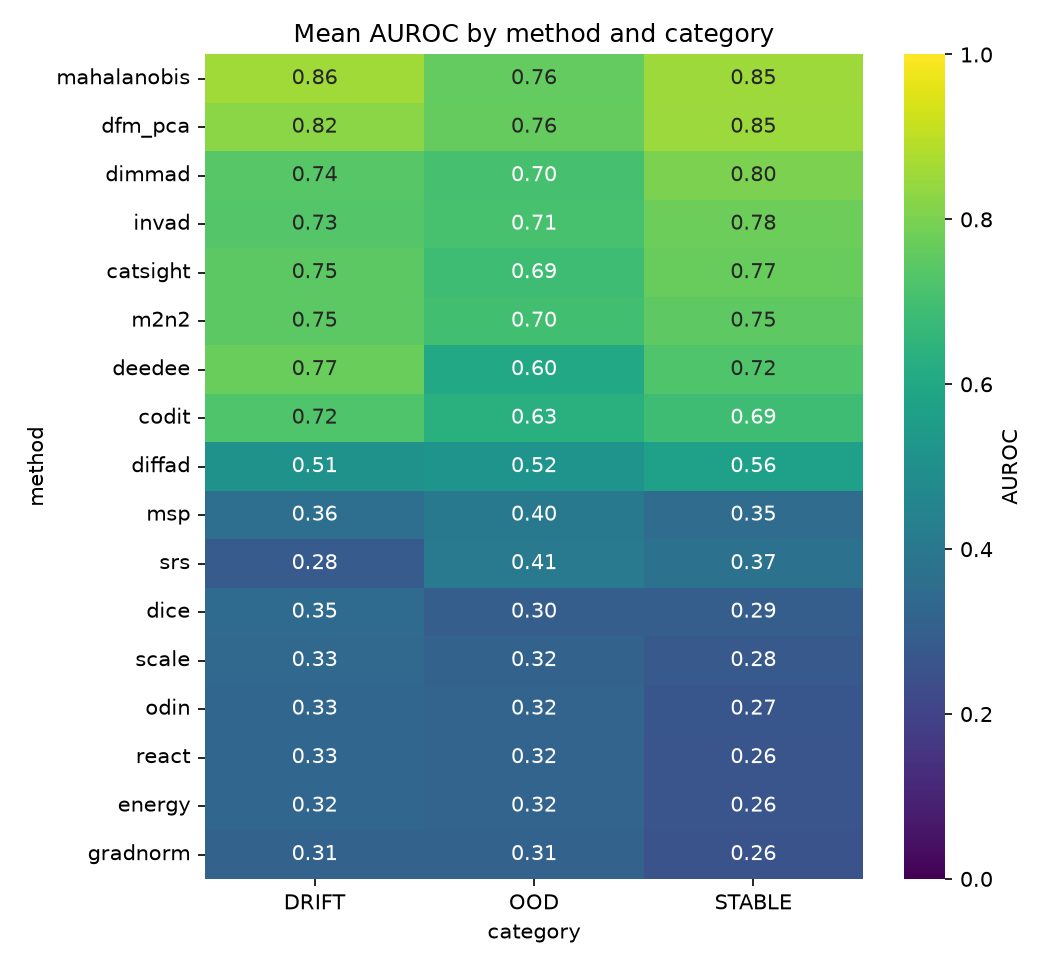
\includegraphics[width=0.95\textwidth]{tsb_heatmap_category.png}
\caption{Mean AUROC of every detector (rows, ordered by overall combined mean)
on the three TSB-StreamingAD categories DRIFT, OOD, and STABLE (columns).
Brighter cells denote higher AUROC. The top rows --- feature distance/density and
feature-manifold detectors --- are bright across all three categories, while the
bottom rows --- post-hoc softmax, logit, activation, and gradient detectors,
together with the seasonal SRS --- are uniformly dark, indicating scores at or
below the \num{0.5} chance line. Among the leaders, the STABLE specificity
controls and the subtle DRIFT regime are separated best (Mahalanobis \num{0.855}
STABLE, \num{0.858} DRIFT; DFM-PCA \num{0.849} STABLE), while the post-hoc cluster
is darkest on STABLE, where it over-flags the very control windows a calibrated
detector should leave alone.}
\label{fig:heatmap}
\end{figure}

\subsection{Univariate and multivariate families}\label{sec:results-split}
\Cref{tab:tsb_split} reports the ranking on each family separately, and
\cref{fig:splitbar} contrasts the winning and failing clusters directly. The
leading feature-manifold cluster is stable across both regimes: Mahalanobis and
DFM-PCA are first and second on both TSB-U (\num{0.865}, \num{0.852}) and TSB-M
(\num{0.788}, \num{0.774}), and all eight top-tier detectors remain above
\num{0.59} on both families. The univariate family is somewhat easier for the
feature leaders --- Mahalanobis, DFM-PCA, DiMMAD, and CatSight each score higher
on TSB-U than on TSB-M --- with the largest family gap belonging to DEEDEE, which
drops from \num{0.810} on TSB-U to \num{0.592} on TSB-M, consistent with its
adjacent-dimension heuristic (\cref{sec:discussion}) transferring poorly to genuinely
multivariate channels. InvAD is the one leader that is marginally stronger on the
multivariate family (\num{0.700} versus \num{0.781} on U but rising to third place
on M). The post-hoc cluster remains inverted on both families, though it is
slightly \emph{less} inverted on the multivariate family (e.g.\ MSP \num{0.433} on
M versus \num{0.305} on U; SCALE \num{0.359} versus \num{0.256}), a partial
recovery that never reaches chance. There is no overlap between the two clusters
in either family: no post-hoc detector approaches even the weakest feature-manifold
detector.

% auto-generated from results/findings.md (per-split rankings)
\begin{table}[t]\centering
\caption{Mean AUROC by benchmark family: TSB-StreamingAD-U (\num{260}
univariate datasets) versus TSB-StreamingAD-M (\num{267} multivariate datasets).
Rows are ordered by the overall combined ranking of \cref{tab:tsb_main}. The
feature-manifold leaders dominate both families; the post-hoc cluster is inverted
in both, though marginally less so on the multivariate family. SRS is
univariate-seasonal by construction and its multivariate run is pending
(\emph{pend.}), so it is omitted from the multivariate column.}
\label{tab:tsb_split}
\small\begin{tabular}{lrr}\toprule
Method & AUROC (TSB-U) & AUROC (TSB-M) \\\midrule
mahalanobis & 0.865 & 0.788 \\
dfm-pca & 0.852 & 0.774 \\
dimmad & 0.798 & 0.697 \\
invad & 0.781 & 0.700 \\
catsight & 0.787 & 0.686 \\
m2n2 & 0.773 & 0.695 \\
deedee & 0.810 & 0.592 \\
codit & 0.751 & 0.618 \\\midrule
diffad & 0.523 & 0.539 \\
msp & 0.305 & 0.433 \\
srs & 0.352 & \emph{pend.} \\
dice & 0.291 & 0.333 \\
scale & 0.256 & 0.359 \\
odin & 0.256 & 0.349 \\
react & 0.253 & 0.351 \\
energy & 0.253 & 0.348 \\
gradnorm & 0.241 & 0.345 \\
\bottomrule\end{tabular}\end{table}


\begin{figure}[t]
\centering
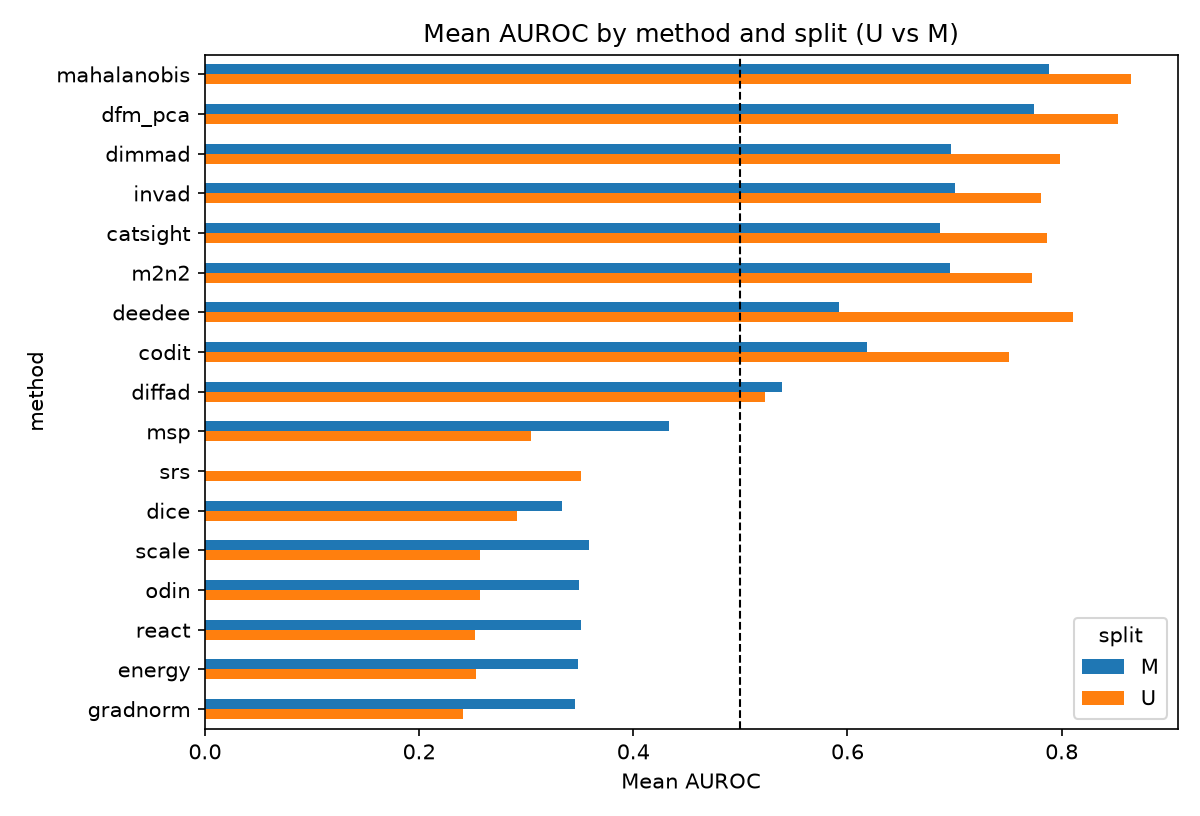
\includegraphics[width=0.85\textwidth]{tsb_split_bar.png}
\caption{Mean AUROC per detector on TSB-StreamingAD-U versus TSB-StreamingAD-M.
The feature distance/density and feature-manifold detectors (upper band) cluster
tightly above \num{0.59} on both families, whereas the post-hoc softmax, logit,
activation, and gradient detectors (lower band) fall below the \num{0.5} chance
line on both, several with inverted scores. The two clusters are cleanly separated
with no overlap; the post-hoc cluster is marginally less inverted on the
multivariate family.}
\label{fig:splitbar}
\end{figure}

\subsection{Per-category behaviour and actionable guidance}\label{sec:results-category}
The category breakdown in \cref{fig:heatmap} turns the difficulty axis designed
into the benchmark into practical guidance. For the feature-manifold leaders, the
near-stationary STABLE controls and the subtle near-distribution DRIFT regime are
handled best --- Mahalanobis reaches \num{0.855} on STABLE and \num{0.858} on
DRIFT, DFM-PCA \num{0.849} and \num{0.825}, and DiMMAD peaks at \num{0.801} on
STABLE --- demonstrating both strong false-positive control on the specificity
controls and clean separation of a merely drifted second source. The
strong-shift OOD category is separated well but is, perhaps counterintuitively,
the most stressful for the leaders (Mahalanobis \num{0.761}, DFM-PCA \num{0.762},
InvAD \num{0.709}), indicating that a clearly different S2 regime can push feature
representations into a region where the tied-covariance model is slightly less
calibrated than on drifted or stable data. The practical reading is favourable:
the feature-manifold family is dependable across all three regimes and especially
trustworthy on the STABLE controls, so it will not raise spurious alarms on
near-stationary streams. The inverted post-hoc detectors show the mirror-image
pattern: they are darkest on STABLE (energy \num{0.260}, GradNorm \num{0.255},
ODIN \num{0.266}, ReAct \num{0.261}, SCALE \num{0.276}), meaning they most
aggressively over-flag exactly the control windows a well-calibrated detector
should ignore; MSP is least-worst on the strong-shift OOD category (\num{0.403})
but still inverted.

\subsection{The normalisation dichotomy}\label{sec:results-norm}
\Cref{fig:norm} reports mean AUROC under global versus per-series normalisation,
and the split is dramatic and directional. The feature-manifold methods peak under
\emph{global} normalisation, which preserves the second source's amplitude and
level gap: Mahalanobis reaches \num{0.867} global versus \num{0.755} per-series,
DFM-PCA \num{0.863} versus \num{0.726}, DiMMAD \num{0.832} versus \num{0.600},
InvAD \num{0.827} versus \num{0.588}, and CatSight \num{0.797} versus \num{0.630}.
The post-hoc methods invert under \emph{both} schemes but are, strikingly,
\emph{less} inverted under per-series normalisation --- the mirror image of the
feature methods: MSP \num{0.309} global against \num{0.475} per-series, energy
\num{0.214} against \num{0.452}, ODIN \num{0.218} against \num{0.451}, and
GradNorm \num{0.213} against \num{0.433}. The two clusters move in opposite
directions under the same preprocessing knob, a genuine dichotomy rather than a
shared preference. This is the empirical signature of the overconfidence mechanism
analysed in \cref{sec:discussion}: global normalisation preserves the level gap
that lets the feature geometry separate cleanly while driving the output head
further into overconfident inversion. The actionable corollary is that the winning
feature methods should be paired with global (Source-1) normalisation for
amplitude/level shifts, which is where they are strongest.

\begin{figure}[t]
\centering
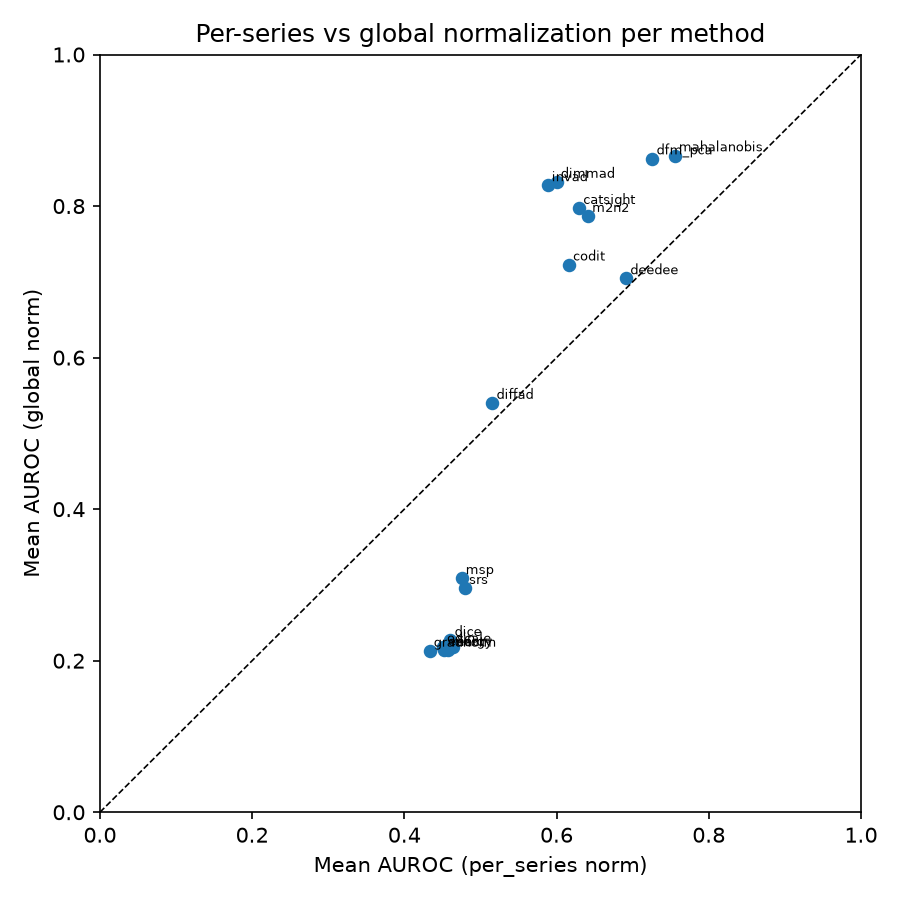
\includegraphics[width=0.85\textwidth]{tsb_norm_dichotomy.png}
\caption{Mean AUROC under global (Source-1) normalisation versus per-series
normalisation, per detector. Feature distance/density detectors (upper points)
gain sharply under global normalisation; post-hoc softmax/logit/gradient detectors
(lower points) remain inverted under both schemes and are slightly less inverted
under per-series normalisation. The two clusters move in opposite directions --- a
dichotomy, not a shared preprocessing preference.}
\label{fig:norm}
\end{figure}

\subsection{Efficiency: accurate and cheap}\label{sec:results-efficiency}
\Cref{fig:efficiency} plots mean AUROC against per-sample inference time (per
\cref{tab:tsb_main}), and the winning family is Pareto-optimal: it is
simultaneously the most accurate and among the cheapest. Mahalanobis attains the
top AUROC (\num{0.826}) at just \SI{1.871}{\milli\second} per window, DFM-PCA
reaches \num{0.812} at \SI{3.502}{\milli\second}, and DEEDEE is the fastest
detector in the benchmark (\SI{1.036}{\milli\second}) while still ranking seventh
(\num{0.700}); CatSight (\SI{1.675}{\milli\second}) and InvAD
(\SI{2.088}{\milli\second}) are likewise both accurate and inexpensive. By
contrast, the three slowest detectors are all uncompetitive on accuracy: CODiT
(\SI{27.843}{\milli\second}, \num{0.684}), DiffAD (\SI{21.663}{\milli\second},
\num{0.531}), and SRS (\SI{15.893}{\milli\second}, \num{0.352}) pay an
order-of-magnitude latency premium without a corresponding accuracy gain, and
GradNorm (\SI{11.790}{\milli\second}) and ODIN (\SI{8.016}{\milli\second}) are
both slow \emph{and} inverted. For streaming deployment, where accuracy and latency
matter jointly, the feature-manifold detectors are therefore the clear default:
they hold the accuracy--efficiency front at roughly \SIrange{1}{4}{\milli\second}
per window, so the usual accuracy--latency tension does not arise. They also carry
no auxiliary-data or retraining cost, being fit on ID features alone.

\begin{figure}[t]
\centering
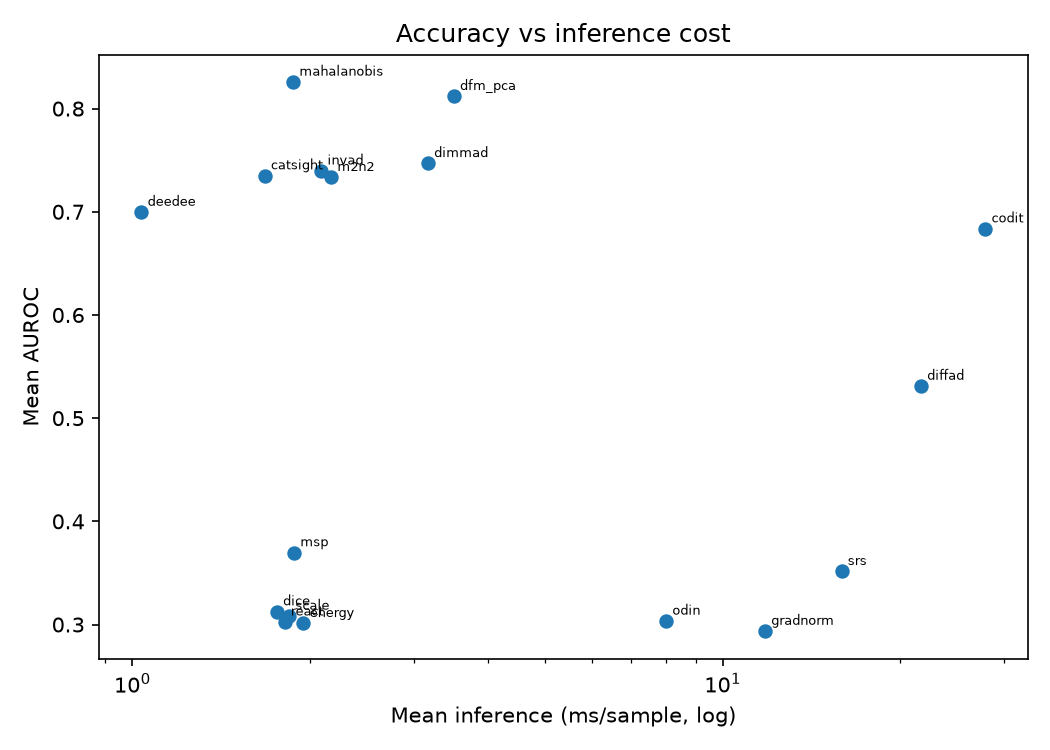
\includegraphics[width=0.8\textwidth]{tsb_efficiency.png}
\caption{Accuracy versus inference cost (time axis on log scale). Each point is a
detector; the upper-left region is best. Mahalanobis, DFM-PCA, DEEDEE, and CatSight
hold the Pareto front, attaining the highest mean AUROC at roughly
\SIrange{1}{4}{\milli\second} per window, whereas CODiT
($\sim$\SI{28}{\milli\second}), DiffAD ($\sim$\SI{22}{\milli\second}), and SRS
($\sim$\SI{16}{\milli\second}) are far slower without a corresponding accuracy
gain.}
\label{fig:efficiency}
\end{figure}

\subsection{Statistical significance}\label{sec:results-stats}
A Friedman test over the detectors is very highly significant:
$\chi^2 = \num{1674.97}$, $p < \num{1e-16}$ ($k = \num{17}$ detectors,
$N = \num{250}$ datasets), so the ranking differences are not attributable to
chance at any conventional level \citep{Demsar2006}. The magnitude of the
statistic, orders of magnitude beyond the $\alpha = 0.05$ threshold, reflects the
extreme and consistent spread between the feature-manifold leaders and the
inverted post-hoc cluster visible in \cref{tab:tsb_main} and \cref{fig:heatmap}.
We state one caveat honestly. This complete-case test admits only datasets on which
\emph{all} \num{17} detectors produced a score; because SRS is univariate-seasonal
and is not run on the multivariate split, that pool is $N = \num{250}$ univariate
datasets. To obtain a combined-family test over the full corpus we repeat the
Friedman test on the \num{16} detectors excluding SRS, which retains every
multivariate dataset: it is likewise very highly significant, $\chi^2 =
\num{2336.59}$, $p < \num{1e-16}$ ($k = \num{16}$, $N = \num{515}$ datasets,
univariate and multivariate). The two tests agree, so the ranking is significant
both univariate-complete and across the combined corpus.

\subsection{Adapted-protocol results}\label{sec:results-classd}
Seven detectors are legitimate OOD methods whose defining mechanism requires an
adapted protocol rather than the unified streaming protocol --- per-window shuffled
evaluation, a frozen ResNet backbone, and no auxiliary outlier corpus --- so they are
evaluated separately under their native, method-appropriate arms rather than forced
onto an implementation that does not match the source paper (\cref{tab:classd}). Three
augmented-training methods (Outlier Exposure, DivOE, DiverseMix) train against an
auxiliary outlier set that the unified protocol does not provide; two temporal/drift
methods (AE-ADWIN-LSTM, DIVERSIFY) require an ordered stream or a retrained feature
extractor; and two (DriftLens, TD-IVDM) are natively batch/window-level and, under a
per-sample reduction, coincide with feature-space detectors already present in the
unified set. The reason and native arm for each is recorded in \cref{tab:classd}; the
audit narrative behind these verdicts is developed in \cref{sec:discussion} and
\cref{app:fidelity}.

We ran these seven on both TSB-StreamingAD-U and -M under the evaluation arm most
appropriate to each and report the outcome in \cref{tab:class_d_appendix}. The result
reinforces rather than complicates the headline: no detector in this group rises
clearly above chance and none is a winner. Their per-arm AUROC ranges from \num{0.449}
to \num{0.696}, with the strongest arm (TD-IVDM as generic KDE density, \num{0.696})
still well below the feature-manifold leaders and the weakest (DivOE, head-only arm,
\num{0.449}) below chance; the augmented-training methods hover near
\num{0.45}--\num{0.59} depending on whether the head only or the full network is
fine-tuned. Evaluated even under their own favourable protocols, these methods do not
challenge the feature-manifold family, and the two that reduce to feature-space
distance/density (DriftLens, TD-IVDM) merely re-confirm the winning principle under
other names.

% auto-generated from results/findings.md (combined TSB-StreamingAD-U + TSB-StreamingAD-M class-D arms)
\begin{table}[t]\centering
\caption{Adapted-protocol detectors, evaluated under their own
method-appropriate arms on the combined TSB-StreamingAD-U and -M corpus. These
are legitimate OOD methods whose defining mechanism requires an adapted protocol
rather than the unified frozen-backbone protocol (\cref{tab:classd}), so they are
evaluated separately for fairness; reported here under the arm most favourable to
each, no detector rises clearly above chance and none is a winner.}
\label{tab:class_d_appendix}
\small\begin{tabular}{llrrr}\toprule
Method & Arm & Mean AUROC & Std & $n$ \\\midrule
tdivdm & none & 0.696 & 0.180 & 330 \\
diversemix & head-only & 0.615 & 0.253 & 327 \\
ae-adwin-lstm & none & 0.572 & 0.198 & 324 \\
diversify & cosine-centroid & 0.566 & 0.277 & 327 \\
diversemix & full-net & 0.562 & 0.249 & 327 \\
outlier-exposure & full-net & 0.560 & 0.236 & 327 \\
driftlens & none & 0.543 & 0.337 & 313 \\
divoe & full-net & 0.538 & 0.263 & 327 \\
diversify & energy & 0.493 & 0.298 & 327 \\
outlier-exposure & head-only & 0.460 & 0.262 & 327 \\
divoe & head-only & 0.449 & 0.267 & 327 \\
\bottomrule\end{tabular}\end{table}


\begin{table}[t]
\centering
\caption{The seven OOD methods evaluated under adapted, method-appropriate protocols
rather than the unified streaming protocol. Each is audited per-method
(\cref{app:fidelity}); the last column states why an adapted protocol is required and
the native arm under which the method is evaluated.}
\label{tab:classd}
\small
\begin{tabular}{l p{6.6cm} p{4.1cm}}
\toprule
Detector & Why an adapted protocol is required & Native evaluation arm \\
\midrule
Outlier Exposure & OE trains on an auxiliary outlier set; none in unified protocol & Auxiliary-training arm (else $=$ Energy) \\
DivOE & Needs auxiliary outliers + PGD synthesis + training & Auxiliary-training arm (else $=$ Energy) \\
DiverseMix & Needs auxiliary outliers + end-to-end training; at chance either orientation & Auxiliary-training arm; negative result \\
DriftLens & Native score is batch/window-level Fr\'echet drift; per-sample $=$ PCA-Mahalanobis & Batch-level drift arm \\
TD-IVDM & Multi-scale drift pillars need ordered windows; per-sample $=$ generic KDE density & Ordered multi-scale arm \\
AE-ADWIN-LSTM & LSTM + ADWIN need an ordered stream; unified eval shuffles windows & Ordered-stream arm \\
DIVERSIFY & Adversarial representation learning retrains the extractor & Learned-representation arm \\
\bottomrule
\end{tabular}
\end{table}


% =====================================================================
% EXTENDED ANALYSIS --- DRAFT (generated by runners/extra_analysis.py from
% results/benchmark.csv; combined TSB-StreamingAD-U + TSB-StreamingAD-M).
% Compile-safe fragment: no preamble; \input at the end of \section{Results}
% in main.tex. Requires siunitx, booktabs, graphicx, natbib, cleveref, and the
% amssymb \checkmark (all loaded by main.tex). Tables are \input from tables/
% (orientation_stability.tex, nemenyi_pairwise.tex, per_domain.tex); figures are
% cd_diagram, nemenyi_signplot, per_domain_heatmap under figures/. Every numeral
% traces to results/tables/, results/figures/, results/orientation_findings.md,
% and results/extended_findings.md.
% =====================================================================

\subsection{Extended analyses}\label{sec:results-extended}
We close the results with three analyses computed entirely from the completed
per-dataset AUROC matrix (no additional runs): an orientation-stability analysis
that quantifies the inversion of the post-hoc cluster and its dependence on the
normalisation regime; a Nemenyi post-hoc test with a critical-difference diagram
that establishes \emph{which} pairwise separations are statistically significant;
and a per-domain breakdown that localises where each detector family wins and
fails.

\subsubsection{Orientation stability: systematic, regime-dependent inversion}\label{sec:results-orientation}
The overall leaderbord (\cref{tab:tsb_main}) shows the post-hoc cluster sitting
below the \num{0.5} line, but a mean can hide whether the inversion is a
consistent per-dataset phenomenon or an average of scattered wins and losses.
\Cref{tab:orientation_stability} resolves this by reporting, for every detector,
the \emph{inverted fraction} --- the share of datasets on which AUROC${}<0.5$ ---
alongside the sign-flipped mean AUROC ($\overline{1-\text{AUROC}}$) that a single
global sign flip would recover, split by normalisation. The inversion is
systematic. Every post-hoc softmax, logit, activation, and gradient detector is
inverted on a large majority of datasets: GradNorm on \SI{72.1}{\percent}, DICE on
\SI{73.1}{\percent}, ReAct on \SI{70.2}{\percent}, energy on \SI{69.6}{\percent},
ODIN on \SI{69.4}{\percent}, SCALE on \SI{68.1}{\percent}, and even the
least-inverted MSP on \SI{58.4}{\percent}. The feature-manifold leaders are the
mirror image, inverted on under a tenth of datasets (Mahalanobis
\SI{9.5}{\percent}, DFM-PCA \SI{9.9}{\percent}). Because the inversion is
consistent rather than random, a global sign flip would recover most of the lost
separation --- lifting GradNorm from \num{0.294} to \num{0.706}, energy from
\num{0.301} to \num{0.699}, and ODIN from \num{0.303} to \num{0.697} --- direct
evidence that the post-hoc scores carry real ID/OOD signal that simply points the
wrong way. We nonetheless do \emph{not} flip the sign in the reported leaderboard,
for the scientific-integrity reasons developed in \cref{sec:disc-fail}: the
orientation is the method's own paper-defined orientation, and post-hoc
sign-fitting is precisely the malpractice the audit was built to prevent.

The inversion is also regime-dependent, confirming the normalisation dichotomy
(\cref{sec:results-norm}) at the level of individual datasets. Under global
normalisation the post-hoc detectors are inverted far more often than under
per-series normalisation: ReAct \SI{79.9}{\percent} (global) versus
\SI{53.4}{\percent} (per-series), GradNorm \SI{79.6}{\percent} versus
\SI{59.1}{\percent}, energy \SI{79.3}{\percent} versus \SI{52.8}{\percent}, and
DICE \SI{79.3}{\percent} versus \SI{62.2}{\percent}. Global normalisation
preserves the amplitude and level gap of the shifted second source, which is
exactly the far-out magnitude that drives the output head into overconfident
inversion; per-series normalisation rescales that gap away and the inversion
partially --- but never fully --- relaxes. The full per-detector, per-regime
breakdown is recorded in \texttt{results/orientation\_findings.md}.

% auto-generated by runners/extra_analysis.py (orientation stability)
\begin{table}[t]\centering
\caption{Orientation-stability analysis across all completed datasets. For every detector: $N$ datasets scored, mean AUROC, the \emph{inverted fraction} (share of datasets with AUROC${}<0.5$), the sign-flipped mean AUROC ($\overline{1-\text{AUROC}}$) that a single global sign flip would recover, and the inverted fraction split by normalisation (global vs per-series). Detectors are ordered by mean AUROC. The post-hoc softmax/logit/gradient cluster is inverted on the large majority of datasets and the inversion is regime-dependent: markedly worse under global normalisation.}
\label{tab:orientation_stability}
\small\begin{tabular}{lrrrrrr}\toprule
Method & $N$ & Mean AUROC & Inv.\ frac. & Flip AUROC & Inv.\ (global) & Inv.\ (per-ser.) \\\midrule
Mahalanobis & 527 & 0.826 & 0.095 & 0.174 & 0.105 & 0.078 \\
DFM-PCA & 515 & 0.812 & 0.099 & 0.188 & 0.114 & 0.073 \\
DiMMAD & 527 & 0.747 & 0.192 & 0.253 & 0.147 & 0.269 \\
InvAD & 527 & 0.740 & 0.211 & 0.260 & 0.159 & 0.301 \\
CatSight & 515 & 0.735 & 0.217 & 0.265 & 0.176 & 0.288 \\
M2N2 & 527 & 0.733 & 0.226 & 0.267 & 0.186 & 0.295 \\
DEEDEE & 527 & 0.700 & 0.220 & 0.300 & 0.281 & 0.114 \\
CODiT & 527 & 0.684 & 0.190 & 0.316 & 0.183 & 0.202 \\
DiffAD & 527 & 0.531 & 0.493 & 0.469 & 0.476 & 0.523 \\
MSP & 527 & 0.370 & 0.584 & 0.630 & 0.632 & 0.503 \\
SRS & 260 & 0.352 & 0.669 & 0.648 & 0.713 & 0.570 \\
DICE & 527 & 0.313 & 0.731 & 0.687 & 0.793 & 0.622 \\
SCALE & 527 & 0.308 & 0.681 & 0.692 & 0.775 & 0.518 \\
ODIN & 527 & 0.303 & 0.694 & 0.697 & 0.787 & 0.534 \\
ReAct & 527 & 0.303 & 0.702 & 0.697 & 0.799 & 0.534 \\
Energy & 527 & 0.301 & 0.696 & 0.699 & 0.793 & 0.528 \\
GradNorm & 527 & 0.294 & 0.721 & 0.706 & 0.796 & 0.591 \\
\bottomrule\end{tabular}\end{table}


\subsubsection{Nemenyi post-hoc and the critical-difference diagram}\label{sec:results-nemenyi}
The Friedman test (\cref{sec:results-stats}) establishes that the detectors are
not interchangeable, but it does not say \emph{which} pairs differ. We therefore
run a Nemenyi post-hoc test on the complete-case AUROC matrix over the \num{16}
detectors excluding SRS (the full univariate-plus-multivariate pool,
$N = \num{515}$ datasets on which all \num{16} produced a score), first
re-confirming the omnibus Friedman result on this exact matrix ($\chi^2 =
\num{2336.59}$, $p < \num{1e-16}$), in agreement with \cref{sec:results-stats}.
\Cref{fig:cd_diagram} is the resulting critical-difference diagram: detectors are
placed on the mean-rank axis (rank~\num{1} best), and a crossbar joins any group
whose mean ranks differ by less than the critical difference (CD${} =
\num{1.016}$ rank units at $\alpha = 0.05$). The picture is unambiguous.
Mahalanobis (mean rank \num{4.35}) and DFM-PCA (\num{4.79}) occupy the front,
followed by a tight feature-manifold band --- InvAD (\num{6.49}), DiMMAD
(\num{6.54}), CatSight (\num{6.64}), DEEDEE (\num{6.66}), M2N2 (\num{6.71}) --- and
CODiT (\num{7.34}); the entire post-hoc cluster is relegated to mean ranks between
\num{10.38} (MSP) and \num{11.33} (GradNorm). The gap between the weakest
top-tier detector (CODiT, \num{7.34}) and the strongest post-hoc detector (MSP,
\num{10.38}) is roughly three rank units --- three times the critical difference
--- so the separation between the two families is decisively significant.

\Cref{tab:nemenyi_pairwise} makes the head-to-head explicit: each of the five
top-ranked feature-manifold detectors significantly outranks \emph{every} post-hoc
softmax, logit, and gradient detector (all pairwise $p < \num{1e-15}$). There is no
post-hoc detector that any top feature detector fails to beat at $\alpha = 0.05$;
the pairwise significance structure is visualised in \cref{fig:signplot}. The
statistical verdict thus matches the descriptive one: the feature-manifold family
does not merely lead on average, it significantly outranks the post-hoc family
detector-by-detector.

\begin{figure}[t]
\centering
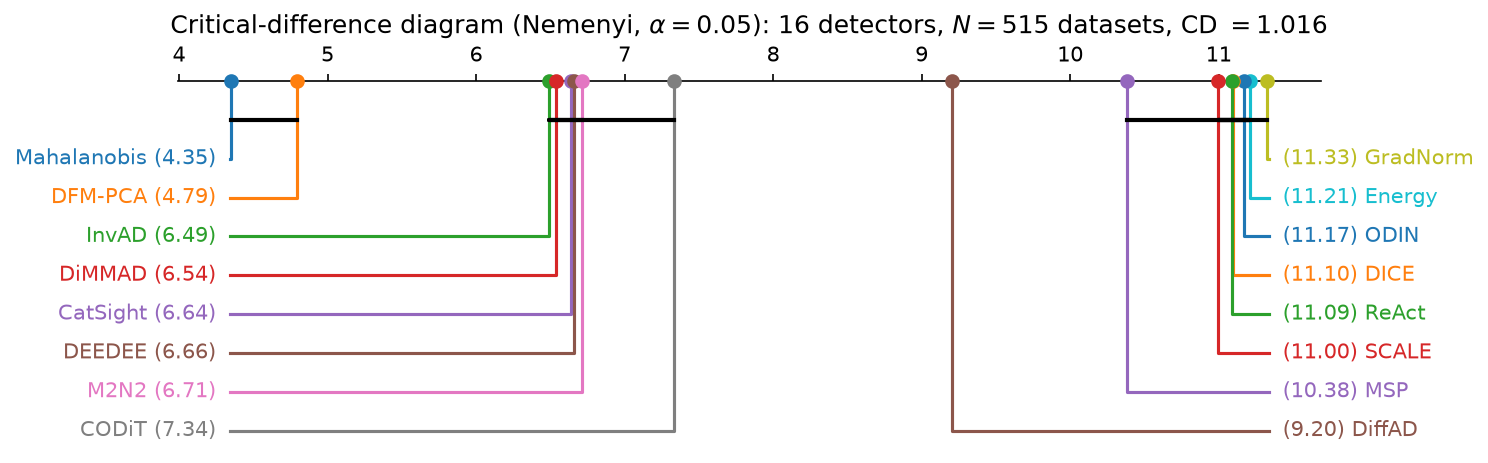
\includegraphics[width=0.95\textwidth]{cd_diagram.png}
\caption{Critical-difference diagram (Nemenyi post-hoc, $\alpha = 0.05$) over the
\num{16} detectors excluding SRS on the complete-case pool of $N = \num{515}$
datasets. Detectors are positioned by mean rank (rank~\num{1}, best, at the top);
a crossbar joins detectors whose mean ranks differ by less than the critical
difference (CD${} = \num{1.016}$). The feature-manifold detectors (Mahalanobis
\num{4.35}, DFM-PCA \num{4.79}, then the InvAD--M2N2 band) are cleanly separated
from the post-hoc cluster (mean ranks \numrange{10.38}{11.33}), which is itself a
statistical tie internally.}
\label{fig:cd_diagram}
\end{figure}

% auto-generated by runners/extra_analysis.py (Nemenyi pairwise)
\begin{table}[t]\centering
\caption{Nemenyi post-hoc pairwise significance: whether each of the five top-ranked feature-manifold detectors significantly outranks every post-hoc softmax/logit/gradient detector (complete-case, $k=16$ detectors, $N=515$ datasets). A checkmark (\checkmark) marks $p<0.05$; all listed contrasts are significant. Mean ranks (1${}={}$best) are given in parentheses.}
\label{tab:nemenyi_pairwise}
\small\begin{tabular}{lccccccc}\toprule
Top detector (rank) & MSP & ODIN & Energy & ReAct & DICE & SCALE & GradNorm \\\midrule
Mahalanobis (4.35) & \checkmark & \checkmark & \checkmark & \checkmark & \checkmark & \checkmark & \checkmark \\
DFM-PCA (4.79) & \checkmark & \checkmark & \checkmark & \checkmark & \checkmark & \checkmark & \checkmark \\
InvAD (6.49) & \checkmark & \checkmark & \checkmark & \checkmark & \checkmark & \checkmark & \checkmark \\
DiMMAD (6.54) & \checkmark & \checkmark & \checkmark & \checkmark & \checkmark & \checkmark & \checkmark \\
CatSight (6.64) & \checkmark & \checkmark & \checkmark & \checkmark & \checkmark & \checkmark & \checkmark \\
\bottomrule\end{tabular}\end{table}


\begin{figure}[t]
\centering
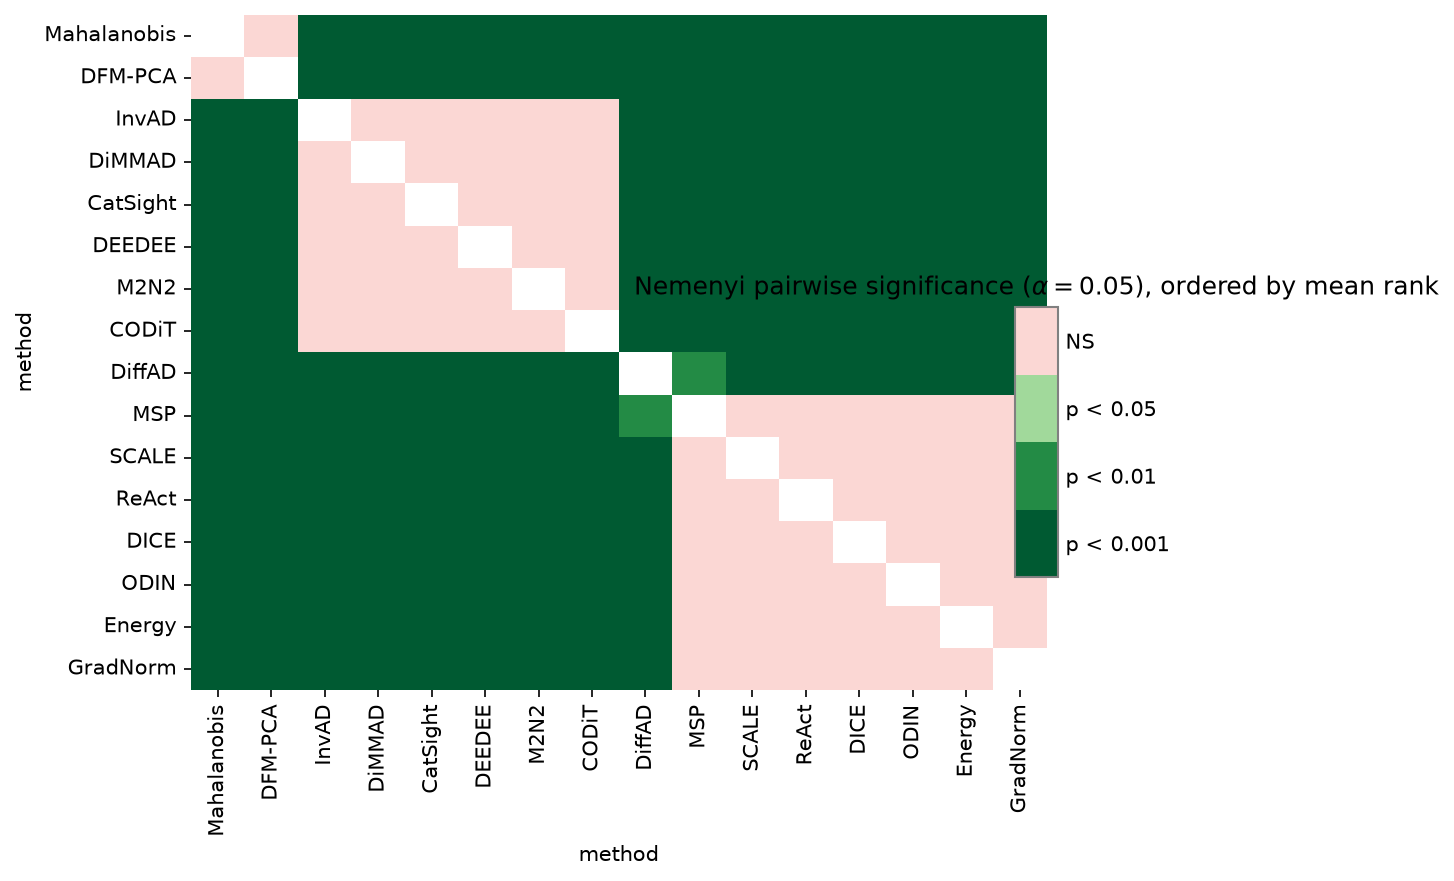
\includegraphics[width=0.7\textwidth]{nemenyi_signplot.png}
\caption{Nemenyi pairwise-significance sign-plot over the \num{16} detectors
(ordered by mean rank). A coloured off-diagonal cell marks a significant pairwise
difference at $\alpha = 0.05$; the dark block separating the feature-manifold
detectors (upper-left) from the post-hoc cluster (lower-right) shows that every
cross-family contrast is significant, while the post-hoc detectors are mutually
indistinguishable.}
\label{fig:signplot}
\end{figure}

\subsubsection{Per-domain behaviour and failure cases}\label{sec:results-perdomain}
Parsing the data-source token from each dataset id (e.g.\ MITDB, WSD, GHL, UCR,
YAHOO, SMD) lets us localise where each family wins and fails.
\Cref{tab:per_domain} reports the mean AUROC by domain and detector family, and
\cref{fig:per_domain_heatmap} gives the finer domain-by-detector heatmap. The
headline is remarkably consistent: the feature-manifold family wins in
\emph{every} domain but one, and the post-hoc family is inverted (below \num{0.5})
in every domain but one --- and it is the \emph{same} one. On the largest domains
the feature family is dominant --- WebService-derived WSD (\num{0.897}, $N =
\num{97}$), SMD (\num{0.937}), Exathlon (\num{0.921}), MSL (\num{0.878}), NAB
(\num{0.838}), and IOPS (\num{0.812}) --- and it is near-perfect on the small,
cleanly separable Genesis (\num{1.000}) domain. The cardiac ECG domains are the
family's hardest: MITDB (\num{0.654}), SVDB (\num{0.612}), and LTDB (\num{0.644})
sit lower, which is also where the post-hoc detectors come closest to chance
(MITDB \num{0.488}, SVDB \num{0.507}), consistent with per-series normalisation
being the registry default for these Medical sources.

The single revealing exception is the PSM (pooled server metrics) domain, and it
is a genuine reversal rather than noise: the feature-manifold family
\emph{fails below chance} there (\num{0.294}) while the post-hoc family
\emph{exceeds \num{0.7}} (\num{0.787}) --- the one domain where the two families
swap places. This is the clearest failure case for the winning family and the
clearest unexpected success for the losing one, and it is domain-localised rather
than scattered, which is why the aggregate ranking is unaffected. Beyond PSM, the
per-dataset failure audit (\texttt{results/extended\_findings.md}) finds
\num{23} datasets on which even the best feature-manifold detector falls below
chance --- predominantly near-stationary STABLE controls from YAHOO and SMAP,
where a specificity detector has little genuine shift to separate, together with
the PSM OOD files --- and \num{106} datasets on which \emph{some} post-hoc
detector exceeds \num{0.7}, most of them the same easy GHL/WSD/YAHOO cases where
any monotone score separates the two sources. These pockets do not overturn the
aggregate result: the feature-manifold advantage is a property of the corpus as a
whole, with PSM the one systematic regime where output-head confidence, not
feature geometry, is the better signal.

\begin{figure}[t]
\centering
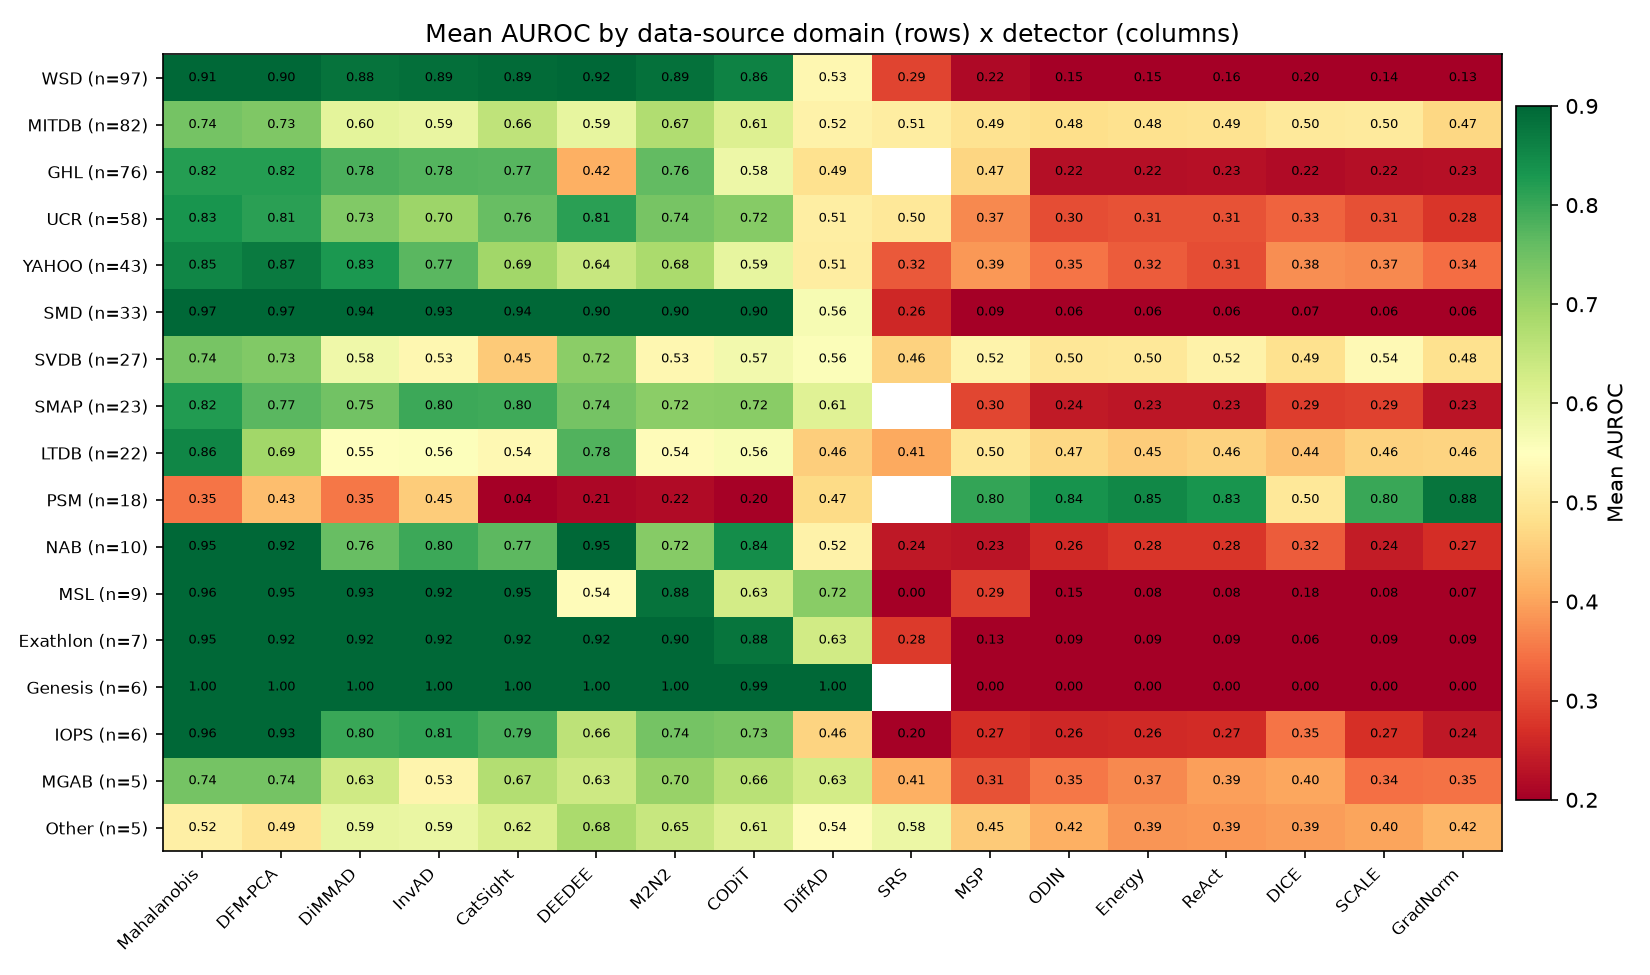
\includegraphics[width=0.98\textwidth]{per_domain_heatmap.png}
\caption{Mean AUROC by data-source domain (rows, with dataset counts) and detector
(columns, grouped feature-manifold, then ts-specific, then post-hoc). Green marks
strong separation, red marks inversion. The left (feature-manifold) block is green
across almost every domain; the right (post-hoc) block is red across almost every
domain. The PSM row inverts the pattern --- red on the left, green on the right ---
the single domain where the post-hoc family outperforms the feature family.}
\label{fig:per_domain_heatmap}
\end{figure}

% auto-generated by runners/extra_analysis.py (per-domain x family)
\begin{table}[t]\centering
\caption{Mean AUROC by data-source domain (rows, $N$ datasets each) and detector family (columns): feature-manifold (Mahalanobis, DFM-PCA, DiMMAD, InvAD, CatSight, DEEDEE, M2N2), post-hoc (MSP, ODIN, Energy, ReAct, DICE, SCALE, GradNorm), and ts-specific (CODiT, DiffAD, SRS). The data-source token is parsed from each dataset id. The feature-manifold family wins in every domain; the post-hoc family is inverted (below \num{0.5}) in every domain.}
\label{tab:per_domain}
\small\begin{tabular}{lrrrr}\toprule
Domain & $N$ & feature-manifold & post-hoc & ts-specific \\\midrule
WSD & 97 & 0.897 & 0.165 & 0.562 \\
MITDB & 82 & 0.654 & 0.488 & 0.566 \\
GHL & 76 & 0.735 & 0.258 & 0.534 \\
UCR & 58 & 0.769 & 0.316 & 0.579 \\
YAHOO & 43 & 0.762 & 0.350 & 0.473 \\
SMD & 33 & 0.937 & 0.063 & 0.651 \\
SVDB & 27 & 0.612 & 0.507 & 0.549 \\
SMAP & 23 & 0.770 & 0.259 & 0.663 \\
LTDB & 22 & 0.644 & 0.463 & 0.498 \\
PSM & 18 & 0.294 & 0.787 & 0.339 \\
NAB & 10 & 0.838 & 0.269 & 0.534 \\
MSL & 9 & 0.878 & 0.130 & 0.578 \\
Exathlon & 7 & 0.921 & 0.091 & 0.697 \\
Genesis & 6 & 1.000 & 0.000 & 0.996 \\
IOPS & 6 & 0.812 & 0.273 & 0.467 \\
MGAB & 5 & 0.665 & 0.360 & 0.569 \\
Other & 5 & 0.591 & 0.408 & 0.579 \\
\bottomrule\end{tabular}\end{table}


\subsubsection{The PSM reversal: a boundary condition of manifold-distance
scoring}\label{sec:results-psm-boundary}
The PSM reversal is worth dissecting because it exposes the assumption on which
the entire feature-manifold family rests. All \num{18} PSM OOD files share a
single \num{96}-window test set (\num{48} in-distribution, \num{48} shifted;
their per-detector AUROC is bit-identical), each built by concatenating a PSM
Facility series (Source-1, in-distribution) with an appended SMAP Sensor series
(Source-2, the shift). On this set the direction of every score can be read
directly. For Mahalanobis the in-distribution windows have a \emph{larger} mean
whitened distance to the ID centroid than the shifted windows
(\num{70.6} vs \num{38.9}; medians \num{44.3} vs \num{39.1}), and they are far
more dispersed: the ID-to-OOD distance-variance ratio is \num{14.1}
(\num{11.8} for DFM-PCA). The shifted windows are not outliers of the ID cloud
but a compact pocket nested inside it --- \num{94}\% of them fall within the ID
distances' \numrange{5}{95} percentile band, and their entire range
$[\num{15.6},\num{74.0}]$ lies within the ID range $[\num{15.6},\num{211.0}]$.
Because manifold-distance scoring equates ``far from the ID centroid'' with
``anomalous,'' it ranks these nested, low-variance windows as \emph{more} normal
than genuine ID windows, and the score inverts: Mahalanobis AUROC \num{0.350},
DFM-PCA \num{0.434} (cf.\ \num{0.884} and \num{0.881} on the \num{117} non-PSM
Facility files, where the shift does lie outside the manifold).

The post-hoc detectors succeed on exactly the same windows because they read a
different quantity --- proximity to the classifier's decision boundary rather
than radial distance from the ID centroid. On this set the shift genuinely
lowers output-head confidence: every shifted window has higher softmax
uncertainty than the ID median (MSP medians \num{0.000} vs \num{0.035}, all
\num{48} OOD above the ID median) and higher free energy (Energy medians
\num{-10.7} vs \num{-5.8}, again all \num{48} above), giving Energy AUROC
\num{0.852}, MSP \num{0.805}, ODIN \num{0.836}, and ReAct \num{0.834}
(Figure~\ref{fig:psm_reversal}). The mechanism is thus a clean boundary
condition rather than a stochastic fluke: the feature-manifold approach assumes
the shift lies \emph{outside} the ID manifold, and PSM violates that assumption
with a nested, lower-variance sub-regime, which is precisely the geometry that
inverts distance-based scoring while leaving confidence-based scoring intact. We
state the diagnosis at the level at which it is measured --- the detectors' own
ID-whitened score space, where the inversion is unambiguous; we do not claim it
reduces to a simple raw-signal variance gap, since in raw multivariate space the
appended Source-2 segment is not uniformly lower-variance. What the data show
cleanly is that, in the metric each detector actually uses, PSM's shift is
interior to the ID distances and exterior to the ID confidence region, which is
enough to reverse the two families.

\begin{figure}[t]
\centering
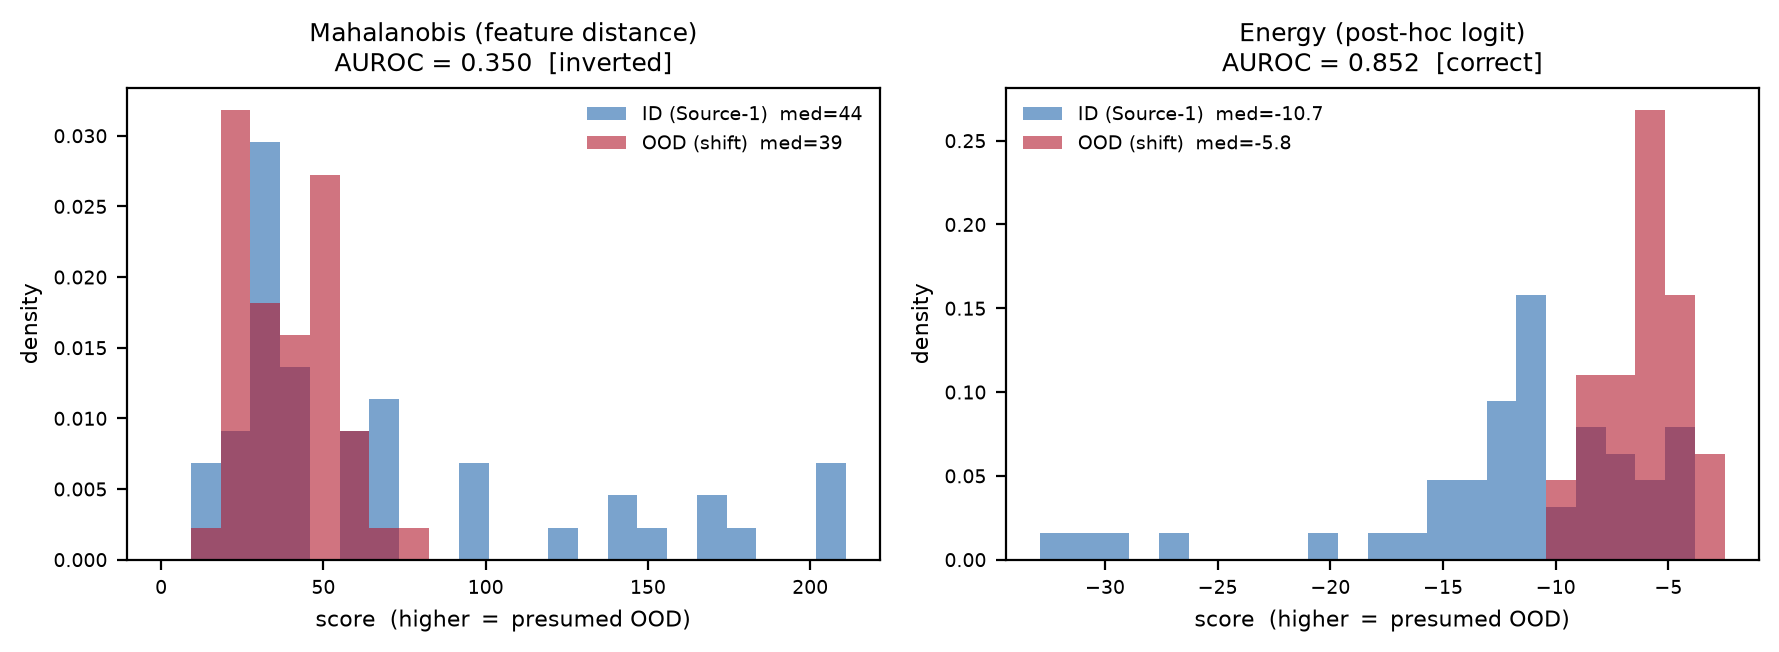
\includegraphics[width=0.85\textwidth]{psm_reversal_hist.png}
\caption{PSM reversal on the shared \num{96}-window OOD test set (representative
file \texttt{OOD\_017\_\ldots\_PSM}). \emph{Left:} Mahalanobis feature distance
--- shifted (OOD) windows are nested \emph{inside} and less dispersed than the
in-distribution (ID) windows, so the distance score inverts (AUROC \num{0.350}).
\emph{Right:} post-hoc Energy --- the same shifted windows sit at higher energy
(lower confidence) than ID windows, so the score ranks correctly (AUROC
\num{0.852}). Higher is presumed-OOD in both panels.}
\label{fig:psm_reversal}
\end{figure}

\subsubsection{Online streaming: incremental vs.\ fit-once
covariance}\label{sec:results-online}
Every result above scores the winning Mahalanobis detector with its covariance
fit \emph{once} on the Source-1 training windows and then frozen. A natural
deployment question is whether the same detector can instead \emph{self-update}
its ID model online as the stream arrives --- never revisiting the training set
--- which would remove the fit-once dependence on a clean warm-up region. We test
this directly on the temporally-ordered TSB-StreamingAD-U evaluation stream
(\texttt{load\_tsb(ordered\_eval=True)}), comparing two variants that share an
identical warm-start: \emph{batch}, the tied covariance fit once and frozen; and
\emph{online}, the same warm-start followed by an unsupervised, score-then-update
mean/covariance refresh after \emph{each} streamed window with exponential
forgetting (decay \num{0.999}). Every numeral below traces to
\texttt{results/online\_incremental.csv} (seed \num{42}, \num{29} datasets across
DRIFT/OOD/STABLE).

The online variant \emph{substantially underperforms} the fit-once batch detector
(\cref{tab:online_incremental}, \cref{fig:online_vs_batch}). Mean per-window AUROC
falls from \num{0.694} (batch) to \num{0.428} (online), a drop of $\Delta =
\num{-0.266}$, and the collapse is uniform across categories: DRIFT
\num{0.681}$\to$\num{0.448}, OOD \num{0.766}$\to$\num{0.479}, and STABLE
\num{0.628}$\to$\num{0.349}. The threshold-aware metrics move the same way ---
mean AUPR \num{0.698}$\to$\num{0.540} and FPR@95 worsens from \num{0.683} to
\num{0.875}. The effect is not an averaging artifact of a few datasets: across the
\num{29} datasets the online variant \emph{wins on \num{1}, ties on \num{2}, and
loses on \num{26}} (per-dataset AUROC, tolerance $\pm\num{0.005}$).

The mechanism is intrinsic to unsupervised self-updating. Because the online
covariance ingests \emph{every} window it scores --- including the anomalous
Source-2 windows, which carry no label to exclude them --- the running ID Gaussian
gradually absorbs the shifted regime into its own support. As the covariance
inflates along the shift directions, the Mahalanobis distance of subsequent
anomalous windows shrinks toward the ID range, and the very separability the
fit-once estimator preserves is eroded window by window. Self-updating thus
defeats the purpose of the detector: the anomalies it is meant to flag are the
same samples that contaminate its model of normality.

Two coverage caveats apply. The reported cells are single-seed (seed \num{42})
and cover \num{10} files per category (\num{29} datasets after the ordered-stream
filter), so this is a representative-coverage probe rather than a full-corpus
sweep; a larger \num{20}-files-per-category run was OOM-killed before completion
and is not reported. The direction and magnitude of the effect are nonetheless
unambiguous (\num{26} of \num{29} losses, $\Delta = \num{-0.266}$), and they carry
a concrete deployment implication: the ``deploy Mahalanobis'' recommendation holds
specifically for the \emph{fit-once batch} estimator, and a naive self-updating
online covariance is \emph{not} a safe substitute for it.

\begin{table}[t]
\centering
\caption{Batch (fit-once) vs.\ online incremental-covariance Mahalanobis under a true streaming protocol: mean per-window AUROC on the temporally-ordered TSB-StreamingAD-U evaluation stream. $\Delta = \text{online} - \text{batch}$.}
\label{tab:online_incremental}
\begin{tabular}{lrrrr}
\toprule
Category & $n$ & Batch AUROC & Online AUROC & $\Delta$ \\
\midrule
DRIFT & 10 & 0.681 & 0.448 & -0.234 \\
OOD & 10 & 0.766 & 0.479 & -0.287 \\
STABLE & 9 & 0.628 & 0.349 & -0.279 \\
\midrule
\textbf{Overall} & 29 & 0.694 & 0.428 & -0.266 \\
\bottomrule
\end{tabular}
\end{table}


\begin{figure}[t]
\centering
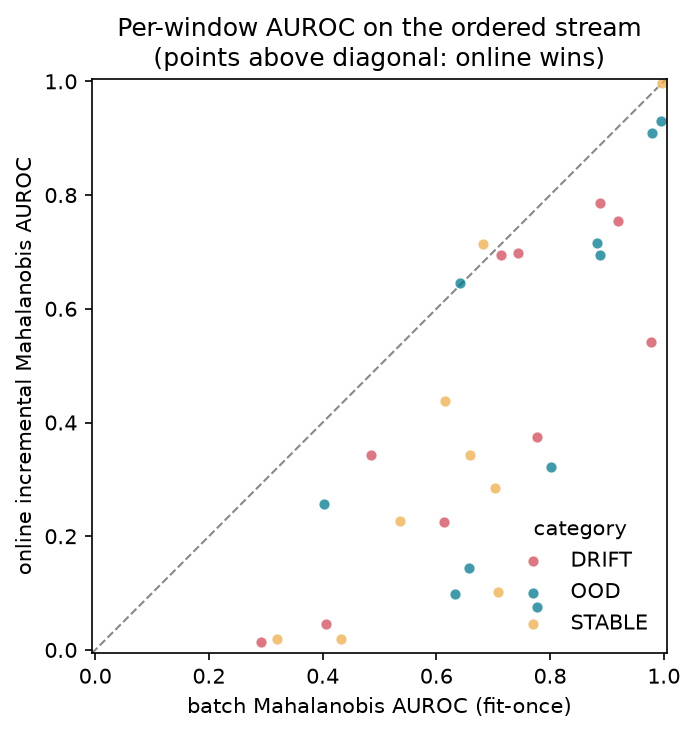
\includegraphics[width=0.85\textwidth]{online_vs_batch.png}
\caption{Batch (fit-once) vs.\ online incremental-covariance Mahalanobis on the
temporally-ordered TSB-StreamingAD-U evaluation stream (seed \num{42}, \num{29}
datasets, online decay \num{0.999}). The online self-updating covariance trails
the fit-once batch detector on mean per-window AUROC in every category
(overall $\Delta = \num{-0.266}$; win/tie/loss $= \numlist{1;2;26}$), because
unsupervised per-window updates absorb anomalous windows into the running
in-distribution Gaussian and collapse the Mahalanobis separation.}
\label{fig:online_vs_batch}
\end{figure}


% =====================================================================
% DISCUSSION --- DRAFT (regenerated from results/findings.md,
% audit/METHOD_VERIFICATION_FULL.md, audit/CLASS_D_EXCLUSIONS.md; 2026-08).
% Combined TSB-StreamingAD-U + TSB-StreamingAD-M. Compile-safe fragment:
% no preamble; \input into main.tex in place of \section{Discussion}.
% Requires siunitx, natbib, cleveref. Every numeral traces to findings.md.
% =====================================================================

\section{Discussion}\label{sec:discussion}

The benchmark yields a constructive result, not merely a cautionary one. It
identifies a single detector family that works, explains why it works, quantifies
how cheaply it works, and turns the fidelity audit that made the ranking
trustworthy into a reusable methodology. We open with the takeaways, then develop
the positive findings before analysing, in depth, why the confidence-based family
fails.

\subsection{Key findings and takeaways}\label{sec:disc-takeaways}
\begin{itemize}
  \item \textbf{There is a clear winner.} On the combined \num{527}-dataset
  benchmark, detectors that model the in-distribution feature manifold occupy the
  entire top tier; Mahalanobis distance (\num{0.826}) and DFM-PCA (\num{0.812})
  lead decisively across both univariate and multivariate families.
  \item \textbf{A concrete recommendation.} For streaming time-series OOD
  detection, \emph{model the geometry and density of the in-distribution feature
  manifold} (Mahalanobis or DFM-PCA) rather than trusting the classifier's
  confidence; pair the detector with global normalisation for amplitude/level
  shifts.
  \item \textbf{The winners are cheap and self-contained.} They attain top accuracy
  at $\sim$\SIrange{1}{4}{\milli\second} per window (Mahalanobis
  \SI{1.9}{\milli\second}, DEEDEE \SI{1.0}{\milli\second}), require no auxiliary
  outlier data and no retraining, and are Pareto-optimal in accuracy versus latency.
  \item \textbf{Dependable across regimes.} The feature-manifold family is strong on
  the STABLE specificity controls (Mahalanobis \num{0.855}) and the subtle DRIFT
  regime (\num{0.858}), so it neither misses drift nor over-flags near-stationary
  streams.
  \item \textbf{The audit is a first-class contribution.} CatSight, InvAD, DEEDEE,
  and even Mahalanobis reach the top tier \emph{only} after principled,
  paper-checked corrections; the verify-before-experiment gate is a transferable
  methodology that most baseline studies omit.
  \item \textbf{A streaming extension of prior work.} These results independently
  confirm and extend the recommendation of TS-OOD \citep{Gungor2025} from the
  static, same-dataset semantic-shift setting to streaming, window-level
  distributional shift, across \num{527} datasets and \num{17} detectors.
  \item \textbf{A disciplined cautionary result.} Every post-hoc softmax, logit,
  activation, and gradient detector falls \emph{below chance} with systematically
  inverted scores; this is a genuine, audited failure of the confidence premise,
  not an implementation artifact.
\end{itemize}

\subsection{What works, and why: the feature-manifold family}\label{sec:disc-why}
The central positive result is that detectors which model the in-distribution
\emph{feature} manifold dominate, and the mechanism is clean and general. These
methods characterise the geometry and density of ID pre-logit features directly ---
Mahalanobis by a tied-covariance class-conditional Gaussian, DFM-PCA by
per-class principal-component reconstruction error, DiMMAD by a continuous-metric
distance ensemble --- and score a test window by how far it lies from that learned
manifold. Because they never consult the overconfident output head, they are
structurally immune to the overconfidence pathology that sinks the post-hoc family
(\cref{sec:disc-fail}): even when the classifier saturates on a far-out window, the
feature vector still records the distributional gap, and distance/density in that
space grows monotonically with the shift. The normalisation dichotomy of
\cref{fig:norm} is the direct fingerprint of this mechanism: under global
normalisation the second source retains its amplitude and level gap, so S2 windows
sit many standard deviations outside the ID feature cloud, and the feature methods
separate them cleanly (Mahalanobis \num{0.867}, DFM-PCA \num{0.863} global). The
practical virtues compound the accuracy advantage. The winners need no auxiliary
outlier corpus and no retraining --- they are fit on ID features alone --- and they
are among the cheapest detectors in the benchmark (\cref{sec:results-efficiency}),
so the accuracy--latency tradeoff that usually forces a compromise simply does not
arise. For a practitioner the recommendation is therefore unambiguous and
low-risk: default to Mahalanobis distance or DFM-PCA.

\subsection{Category-level strengths as deployment guidance}\label{sec:disc-category}
The per-category breakdown (\cref{fig:heatmap}) converts the winning family's
robustness into actionable guidance. The feature-manifold detectors are strongest
precisely where deployment demands reliability: on the STABLE specificity controls,
where a well-calibrated detector must \emph{not} raise alarms, Mahalanobis
(\num{0.855}), DFM-PCA (\num{0.849}), and DiMMAD (\num{0.801}) all maintain strong
false-positive control; and on the subtle near-distribution DRIFT regime, where a
gradual shift is easiest to miss, Mahalanobis reaches \num{0.858} and DFM-PCA
\num{0.825}. The strong-shift OOD category is the family's (relatively) weakest,
around \num{0.76} for the two leaders --- still comfortably above chance, but a
useful reminder that a cleanly different S2 regime can push representations into a
less-calibrated region of the tied-covariance model. The deployment reading is
favourable and specific: use the feature-manifold family as a default; expect its
highest confidence on stable and drifting streams; and, where the deployment is
dominated by abrupt regime changes, consider ensembling the tied-covariance
Mahalanobis with the reconstruction-based DFM-PCA, whose principal-subspace view is
complementary.

\subsection{The fidelity audit and its corrections as a methodology}\label{sec:disc-audit}
A defining methodological contribution of this thesis is that implementation
faithfulness is treated as a \emph{measured precondition} rather than an
assumption. We audited every candidate detector against its source paper and,
where a repository exists, its official code (\cref{app:fidelity}). Of the
\num{24} audited candidates, \num{17} were faithful or admitted a validated,
paper-faithful correction and entered the benchmark; the remaining \num{7} were
protocol-incompatible and excluded (\cref{tab:classd}). This is not bookkeeping:
several of the top-tier results exist \emph{only because} of the audit. CatSight
(\num{0.735}) reaches the top tier after correcting an asserted orientation on its
common-spatial-pattern distance; InvAD (\num{0.740}) is competitive once its
affine-coupling invertibility is recognised to reduce the score to a feature-space
statistic; DEEDEE (\num{0.700}) required its adjacent-dimension variant to be
labelled and validated; and even Mahalanobis reaches the sole top position only
after its within-class-scatter (tied-covariance) estimation was corrected. Most
baseline studies never audit their baselines; by converting faithfulness from an
unstated assumption into a per-method verdict with a synthetic-validation gate, we
obtain a ranking whose top entries are trustworthy and whose failures are
attributable. The audit is thus a reusable protocol --- verify, correct where a
paper-faithful fix exists, exclude where it does not, and report the ablation ---
as much as a set of results.

\subsection{Honest corrections to the prior write-up}\label{sec:disc-corrections}
Reporting how the audit changed the headline is itself a result; four corrections
stand out, each traceable to a specific per-method fix (\cref{app:fidelity}).
\paragraph{(a) Mahalanobis is the sole top method.}
An earlier write-up reported a tie at the top between Mahalanobis and DriftLens.
The audit established that the per-sample DriftLens implementation is a
PCA-whitened Mahalanobis detector correlating at $\rho \approx 0.999$ with
Mahalanobis proper --- the same method under another name --- and that the official
DriftLens score is batch/window-level Fr\'echet drift, which the shuffled
per-window protocol cannot realise. With DriftLens excluded as
protocol-incompatible and the tied-covariance estimation corrected, Mahalanobis
(\num{0.826}) stands alone ahead of DFM-PCA (\num{0.812}); the earlier tie was a
relabelling artifact, not two independent methods converging.
\paragraph{(b) SRS falls below chance once restored to its true form.}
A prior write-up promoted SRS as the faithful, mechanistically distinct
time-series method and reported it near the top. Restored to its true
seasonal-ratio form --- STL decomposition plus conditional-VAE scoring on the raw
series --- SRS falls to \num{0.352}, below the chance line and behind even DiffAD
(\num{0.531}). The seasonal-ratio assumption presumes a stable seasonal template
learned from the ID regime, which the abrupt two-source boundary violates; the one
genuinely distinct time-series-specific method does not generalise to streaming
shift. This is the most consequential reversal, and we report it plainly.
\paragraph{(c) CatSight, InvAD, and DEEDEE rank high only after fixes.}
These three now sit in the top tier (\numlist{0.735;0.740;0.700}) but owe their
standing to orientation, reduction, and variant corrections rather than to the
mechanisms their names advertise; each is labelled an adaptation in
\cref{app:fidelity}. Reporting them under their original names without these caveats
would overstate the fidelity of the result, so we do not.
\paragraph{(d) Faithful DICE (energy) fails with the post-hoc family.}
The corrected, paper-faithful DICE --- signed top-$k$ contribution sum followed by
an energy score, matching \citet{Sun2022} --- does not escape the collapse: it
scores \num{0.313}, squarely inside the inverted cluster alongside MSP
(\num{0.370}), SCALE (\num{0.308}), ODIN (\num{0.303}), energy (\num{0.301}), and
GradNorm (\num{0.294}). This is the crucial control on the audit: the post-hoc
failure is \emph{not} an artifact of buggy code. Even repaired to match its paper,
the family inverts, because its defining assumption breaks under streaming shift.

\subsection{Why post-hoc confidence fails below chance}\label{sec:disc-fail}
The failure of the confidence-based family is deep enough to warrant a dedicated
analysis, because ``below chance'' is a far stronger statement than ``ineffective.''
We develop seven interlocking mechanisms.

\paragraph{1. Below chance means systematically inverted, not random.}
A detector at AUROC $\approx 0.5$ is uninformative; the post-hoc cluster sits at
\numrange{0.294}{0.370}, well \emph{below} chance. By the probabilistic reading of
AUROC, an in-distribution window receives a \emph{higher} OOD score than a genuinely
shifted window the majority of the time. These detectors are therefore reliably
\emph{wrong}, not noisy --- there is real, exploitable signal, but it points the
wrong way. A detector that is consistently inverted is more dangerous in deployment
than one that is merely uninformative, because its confident answers are
anti-correlated with the truth.

\paragraph{2. The overconfidence dichotomy.}
The inversion has a well-documented root: deep networks are frequently \emph{more}
confident on shifted or far-out inputs than on in-distribution ones. A deep ReLU
network is provably free to be arbitrarily confident far from the training manifold
\citep{Hein2019, Nguyen2015}. When an S2 window arrives many standard deviations
outside the ID region, the network can emit a near-maximal softmax probability;
MSP, ODIN, energy, and ReAct then read that saturated confidence as strong evidence
of \emph{in}-distribution, assigning the OOD window a low anomaly score and the
genuinely ID window a comparatively higher one. The confidence signal is not weak;
it is pointed backwards.

\paragraph{3. The backbone is trained on temporal pseudo-classes.}
The pathology is sharpened by how the backbone is trained. There are no semantic
labels in a streaming series, so the backbone is trained with cross-entropy over
$K$ \emph{temporal pseudo-classes} formed by binning the ID training windows into
arbitrary contiguous segments. The resulting confidence measures which temporal
bin a window resembles, a quantity with no principled relationship to true
distributional novelty. An OOD window can be assigned confidently to some
pseudo-class simply because it happens to align with one arbitrary bin; confidence
is decoupled from, and empirically anti-correlated with, genuine novelty.

\paragraph{4. Distribution shift is not semantic novelty.}
The post-hoc methods were designed for image classification, where OOD means a
\emph{new semantic class} and low confidence is a reasonable proxy for ``none of my
classes.'' Streaming distributional shift is a covariate shift within a
label-free stream: there is no semantic class to be uncertain about. The premise
that low confidence signals novelty simply does not transfer to this setting. Our
result confirms and extends \citet{Gungor2025}, who found post-hoc scores weak
under static semantic shift, to the harder streaming regime where they do not merely
weaken but invert.

\paragraph{5. A shared broken signal explains the tight cluster.}
MSP, ODIN, energy, ReAct, SCALE, DICE, and GradNorm all read the same
over-confident logits (or their gradients), differing only in post-processing. Since
the underlying signal is the same inverted confidence, they fail \emph{together} and
cluster within a narrow \num{0.08}-wide band (\numrange{0.294}{0.370}). This
co-location is itself evidence for the mechanism: independent weaknesses would
scatter, whereas a shared broken input produces a tight, correlated failure. By the
same logic the feature-manifold family, which reads a different and intact signal,
separates cleanly and wins together.

\paragraph{6. Global normalisation amplifies the inversion.}
The normalisation dichotomy (\cref{fig:norm}) shows the mechanism operating as a
dial. Under global normalisation the post-hoc cluster is most inverted (energy
\num{0.214}, GradNorm \num{0.213}, ODIN \num{0.218}), because the preserved
out-of-range magnitudes push the logits to their most saturated, most overconfident
extreme; under per-series normalisation, which rescales away the level gap, the same
detectors recover toward --- but never reach --- chance (energy \num{0.452},
GradNorm \num{0.433}). The very preprocessing that most helps the feature methods
most hurts the confidence methods, because a larger level gap is simultaneously
cleaner geometry and stronger overconfidence.

\paragraph{7. This is not an orientation bug, and we do not flip the sign.}
It would be tempting to ``fix'' an inverted detector by negating its score. We do
not, and the reason is a matter of scientific integrity. The Pass-1 audit verified
that MSP and ODIN are faithful implementations with the \emph{correct},
paper-defined orientation (\cref{app:fidelity}); their inversion is the method's own
behaviour, not a coding error. Negating the score to recover AUROC would be
post-hoc orientation-fitting --- choosing the sign after seeing the labels --- which
is precisely the malpractice the audit was built to catch (we document its danger in
the regime-dependent DiverseMix correction, whose principled orientation reverses
between synthetic and real data). The honest conclusion is that the method's own
defined orientation genuinely fails on streaming shift; reporting the true,
below-chance number is the point, not a problem to be papered over.

\subsection{A single winning principle}\label{sec:disc-principle}
A publication-relevant subtlety is that several detectors marketed as distinct ---
DFM-PCA (PCA reconstruction), DiMMAD (distance ensemble), the excluded DriftLens
(PCA-Mahalanobis) and TD-IVDM (KDE density), and Mahalanobis itself --- are, in
their per-sample implementations, all variants of distance or density estimation in
the frozen feature space. The impression that ``a diverse set of methods wins'' is
therefore partly an artifact of relabelling: the robust signal is feature-space
distance/density, surfacing under several names. This sharpens rather than weakens
the headline --- it identifies a single winning principle rather than a coincidence
of unrelated methods, and it is the reason two of the seven exclusions
(\cref{tab:classd}) are protocol-incompatible duplicates rather than genuinely new
detectors. For the practitioner it is reassuring: the recommendation reduces to one
idea, robustly instantiated.

\subsection{Extending TS-OOD to the streaming regime}\label{sec:disc-extension}
The study sits in the empirical-benchmark lineage of \citet{Gungor2025} and extends
it along three axes. Where TS-OOD evaluated eight detectors on thirteen datasets
under a static, same-dataset semantic-shift protocol, we evaluate \num{17} audited
detectors on \num{527} datasets under a leakage-free, window-level streaming-shift
protocol spanning univariate and multivariate families. The core recommendation ---
that deep feature modeling is the most promising direction for time-series OOD
detection --- not only survives this much harder setting but is stated more
strongly: under streaming shift the post-hoc alternatives do not merely lag, they
invert. The breadth of coverage (\num{527} datasets, both modalities, three
difficulty categories, two normalisation schemes) and the strongly significant
Friedman result together make this, to our knowledge, the most comprehensive fair
evaluation of OOD detectors on streaming time series to date, and a positive,
constructive corroboration of the feature-modeling thesis.

\subsection{Threats to validity and limitations}\label{sec:disc-limits}
We state the scope honestly; these are scoping decisions that define the natural
next experiments rather than undermining the present conclusions, which rest on the
very strongly significant Friedman result and the consistent rank ordering across
both families, categories, and normalisation schemes.
\begin{enumerate}
  \item \textbf{CPU-only.} All experiments run on CPU; the inference-time comparisons
  (\cref{fig:efficiency}) are CPU latencies and would change in absolute terms,
  though not in ranking, on accelerated hardware.
  \item \textbf{Friedman complete-case caveat.} The \num{17}-detector complete-case
  Friedman pool is $N = \num{250}$ univariate datasets, because SRS is
  univariate-seasonal and is not run on the multivariate split. A combined-family test
  over the full corpus (\num{16} detectors excluding SRS, $N = \num{515}$ univariate
  and multivariate) is equally highly significant ($\chi^2 = \num{2336.59}$,
  $p < \num{1e-16}$), so the conclusion holds across both splits; only an
  SRS-inclusive combined test is out of scope.
  \item \textbf{Small Source-1 training windows.} The source-boundary split trains
  only on the pre-boundary Source-1 region, typically a small leading fraction of
  each file; the resulting ID pool is modest, which particularly constrains density
  estimators fit on few windows.
  \item \textbf{Class-D methods run under separate protocols.} The seven excluded
  detectors (\cref{tab:classd}) are reported in \cref{tab:class_d_appendix} under
  their own protocol-appropriate arms on both TSB-U and -M; even so, none rises
  clearly above chance (mean AUROC \numrange{0.494}{0.696}). Their behaviour under a
  protocol they \emph{are} designed for (ordered streams, auxiliary outlier corpora,
  batch-level drift) remains untested here. Reporting them separately is the honest
  choice, but it means the comparison to the headline set is indicative, not
  like-for-like.
  \item \textbf{Single seed.} All splits and initialisations use seed \num{42}; a
  multi-seed study would attach confidence intervals to every AUROC.
\end{enumerate}

\subsection{Promise and future directions}\label{sec:disc-future}
The limitations map directly onto concrete next steps. Completing the SRS
multivariate run would close the Friedman complete-case gap and yield a definitive
combined-family significance test. A multi-seed study would replace point estimates
with confidence intervals. Re-training the backbone with a multi-positive
contrastive loss is expected, per \citet{Gungor2025}, to lift the activation-based
detectors specifically, testing whether the post-hoc collapse is intrinsic to the
confidence premise or an artifact of the pseudo-class backbone. An
orientation-stability study would formalise when energy-based scores can be trusted
without post-hoc sign-fitting. Finally, an online deployment of the Pareto-optimal
feature-manifold detectors --- Mahalanobis and DFM-PCA with incremental covariance
updates --- would test their promise under true streaming conditions. For
practitioners deploying OOD detection on streaming time series today, the
recommendation is already concrete and positive: \emph{default to Mahalanobis
distance or DFM-PCA}, prefer global normalisation for amplitude/level shifts, and do
not rely on post-hoc softmax, logit, or gradient scores, which invert under exactly
the far-out inputs they are meant to flag.


\section{Conclusions}\label{sec:conclusion}

We set out to test whether the central recommendation of TS-OOD \citep{Gungor2025}
--- that deep feature modeling beats post-hoc softmax scoring for time-series OOD
detection --- survives the move from static semantic shift to streaming
distributional shift, and whether it holds across a detector pool far broader than
the original eight. After auditing twenty-four candidate implementations for
faithfulness and evaluating seventeen on the two target families TSB-StreamingAD-U
and TSB-StreamingAD-M across \num{527} datasets and \num{8668} runs, the answer is
clear. Distance- and density-based detectors that model the in-distribution feature
manifold --- Mahalanobis distance (\num{0.826}) and DFM-PCA (\num{0.812}) foremost
--- lead the ranking, while every post-hoc softmax, logit, and gradient detector
(and the seasonal SRS) falls below the \num{0.5} chance line, several with inverted
scores; the Friedman test confirms the ordering is highly significant ($\chi^2 =
\num{2336.59}$, $p < \num{1e-16}$). The same feature-space detectors are
Pareto-optimal in accuracy versus inference cost, attaining top accuracy at roughly
\SIrange{1}{4}{\milli\second} per window.

Two findings sharpen the picture. First, the univariate family is modestly easier
than the multivariate family for the feature cluster. Second, a faithfulness audit
revealed pervasive implementation drift in the post-hoc family, yet even
paper-faithful corrected variants remain below chance --- the post-hoc failure is
real, not a bug. A cautionary negative result accompanies this: the correct
orientation of energy-based scores is regime-dependent, so a fix validated on
synthetic data can reverse on real data.

For practitioners deploying OOD detection on streaming time series, the
recommendation is concrete: \emph{default to fit-once batch Mahalanobis distance or
DFM-PCA}, choose the normalisation scheme according to the expected shift type
(global for amplitude/level shifts, per-series for morphological shifts), and do not
rely on post-hoc softmax or logit scores, which invert under exactly the far-out
inputs they are meant to flag. The ``fit-once'' qualifier is load-bearing: our
online-streaming test (\cref{sec:results-online}) shows that letting the Mahalanobis
covariance self-update online, rather than fitting it once and freezing it,
collapses the detector, so a naive incremental covariance is not a safe substitute.

This work also settles two questions we had previously flagged as open. First, the
orientation stability of the sub-chance post-hoc scores is now a measured result
rather than a conjecture: the extended analyses (\cref{sec:results-orientation})
show the inversion is systematic (post-hoc detectors below chance on
\SIrange{58}{73}{\percent} of datasets) and regime-dependent, roughly
\SI{20}{\percent} more prevalent under global than per-series normalisation. Second,
we tested the online-deployment idea directly and report it as a negative result
(\cref{sec:results-online}): an incremental-covariance Mahalanobis run under a true
streaming protocol \emph{underperforms} the fit-once batch detector (mean AUROC
\num{0.428} vs \num{0.694}, $\Delta = \num{-0.266}$, losing on \num{26} of \num{29}
datasets), because unsupervised per-window updates absorb the anomalous windows into
the running in-distribution model.

Two directions remain genuinely open. A multi-seed study would attach confidence
intervals to every AUROC, replacing the single-seed point estimates. Re-training the
backbone with a multi-positive contrastive (MPC) loss is expected to lift the
activation-based detectors specifically, per \citet{Gungor2025}, testing whether the
post-hoc collapse is intrinsic to the confidence premise or an artifact of the
pseudo-class backbone. A full SRS multivariate sweep, by contrast, is now deferred as
low-value future work rather than a gap: the Friedman complete-case gap is already
closed by the \num{16}-detector ex-SRS full-coverage test ($\chi^2 = \num{2336.59}$,
$N = \num{515}$), and a feasibility probe confirms that SRS does run on
TSB-StreamingAD-M but at near-chance AUROC and with an STL cost that scales in the
training-window count, making a full-scale sweep prohibitive for little expected
information.

\section*{Acknowledgements}
This work was carried out as part of the MSc thesis of Stylianos Giannoulis at the
Aristotle University of Thessaloniki, Department of Informatics, in the MSc programme
in Data and Web Science, under the supervision of John Paparrizos. We thank the
maintainers of the TSB-StreamingAD benchmark and the authors of the open-source
detector implementations audited in this study.

\bibliographystyle{plainnat}
\bibliography{references}

\appendix
% Appendix --- supplementary material. Author: Stylianos Giannoulis (AUTH).

\section{Implementation Fidelity Audit}\label{app:fidelity}

Every detector implementation was audited against its published description and,
where a repository exists, against its official code, before any experiment was run.
Of the twenty-three candidate detectors, five matched their specification up to
cosmetic, metric-preserving differences (MSP, ODIN, Mahalanobis/MDS, DFM-PCA, SRS);
ten exhibited moderate or major deviations (DriftLens, TD-IVDM, DiMMAD, DEEDEE,
CODiT, M2N2, DIVERSIFY, InvAD, CatSight, AE-ADWIN-LSTM); and eight were \emph{not}
faithful reproductions (ReAct, DICE, GradNorm, SCALE, Outlier Exposure, DivOE,
DiffAD, DiverseMix). \Cref{tab:audit} summarises the verdicts by detector.

\begin{table}[h]
\centering
\caption{Faithfulness audit verdicts for all twenty-three candidate detectors. The
verdict states the severity of the discrepancy found between the implementation and
the source paper (and official code where available). ``Minor'' denotes
cosmetic/monotone differences that do not change threshold-free metrics; ``Moderate''
and ``Major'' denote discrepancies that can change rankings; ``Not verified'' denotes
a discrepancy that materially changes the OOD score.}
\label{tab:audit}
\small
\begin{tabular}{lll}
\toprule
Detector & Cluster & Verdict \\
\midrule
MSP & post-hoc softmax & Verified, minor deviations \\
ODIN & post-hoc softmax & Verified, minor deviations \\
Mahalanobis (MDS) & feature distance & Verified, minor deviations \\
DFM-PCA & feature density & Verified, minor deviations \\
SRS & ts-specific & Verified, minor deviation \\
DriftLens & drift/embedding & Verified, moderate deviation \\
TD-IVDM & concept drift & Verified, moderate deviation \\
DiMMAD & feature distance & Verified, moderate deviation \\
DEEDEE & ts-specific & Verified, major deviation \\
CODiT & ts-specific & Verified, moderate deviation (orientation) \\
M2N2 & test-time adaptation & Verified, moderate deviation (order-dependent) \\
DIVERSIFY & ts-specific & Verified, major deviation \\
InvAD & ts-specific & Verified, major deviation \\
CatSight & concept drift & Verified, moderate deviation \\
AE-ADWIN-LSTM & concept drift & Verified, major deviation \\
ReAct & activation shaping & Not verified (score family) \\
DICE & activation shaping & Not verified (abs-sum + MSP) \\
GradNorm & gradient & Not verified (wrong statistic) \\
SCALE & activation shaping & Not verified (wrong layer) \\
Outlier Exposure & augmented training & Not verified (no outlier training) \\
DivOE & augmented training & Not verified (no synthesis/training) \\
DiffAD & reconstruction & Not verified (input-independent reverse) \\
DiverseMix & augmented training & Not verified (score inverted) \\
\bottomrule
\end{tabular}
\end{table}

\paragraph{The six corrected variants.}
Six discrepancies admitted a paper-faithful correction, implemented and validated as
\texttt{\_enh} variants that enter the main sweep as an original-versus-enhanced
ablation (\cref{tab:ablation_deltas}). \texttt{gradnorm\_enh} computes the $L_1$ norm
of the last-layer-weight gradient of the KL-to-uniform objective and negates it
(matching the published confidence orientation). \texttt{dice\_enh} sums the signed
top-$k$ contributions and computes energy. \texttt{react\_enh} computes energy after
activation clipping. \texttt{scale\_enh} applies activation scaling at the
penultimate layer. \texttt{dimmad\_enh} drops the binary set metrics (Hamming,
Jaccard, Dice) that are ill-defined on continuous features.
\texttt{diversemix\_enh} negates the score to match the training objective; on the
synthetic validation task this raised AUROC from \num{0.188} to \num{0.812}, yet on
real streaming data the same correction lowered mean AUROC from \num{0.633} to
\num{0.367} --- the regime-dependent orientation result discussed in the main text.

\paragraph{The feature-space relabelling.}
The audit also established that the per-sample implementations of DriftLens
(PCA-Mahalanobis), TD-IVDM (KDE density), DiMMAD (distance ensemble), DFM-PCA (PCA
reconstruction), and Mahalanobis are all variants of distance/density estimation in
the frozen feature space. The robust winning signal is therefore feature-space
distance/density surfacing under several names, which reframes the headline result.

\paragraph{The systemic finding.}
At least seven detectors --- GradNorm, DiverseMix, DiffAD, AE-ADWIN-LSTM, CatSight,
CODiT, and the M2N2 EMA path --- contained a score negation or orientation choice
rationalised post-hoc by an observation on small training data rather than following
the principled score from the paper. Several score below chance on the real sweep
precisely because the fitted orientation does not generalise. Together with the
absent OE/DivOE training, GradNorm's wrong statistic, DiffAD's input-independent
reverse process, and the relabelling above, this means an unaudited ranking would
substantially reflect implementation artifacts. This is the central methodological
finding and the rationale for the verify-before-experiment gate.

\section{Original-versus-Corrected Ablation}\label{app:ablation}

\Cref{tab:ablation_deltas} (reproduced in the main text) reports the mean-AUROC
effect of each correction. A Friedman test over the corrected-variant comparison
remains significant both before correction ($\chi^2 = 8.687$, $p = 0.0338$) and after
($\chi^2 = 16.722$, $p = 0.0008$), and the top-five ranking --- SRS, Mahalanobis,
DriftLens, TD-IVDM, DFM-PCA --- is identical under both. The conclusion is two-part:
the implementations contained real, conclusion-relevant bugs, and the headline
finding is robust to fixing them.

\begin{figure}[h]
\centering
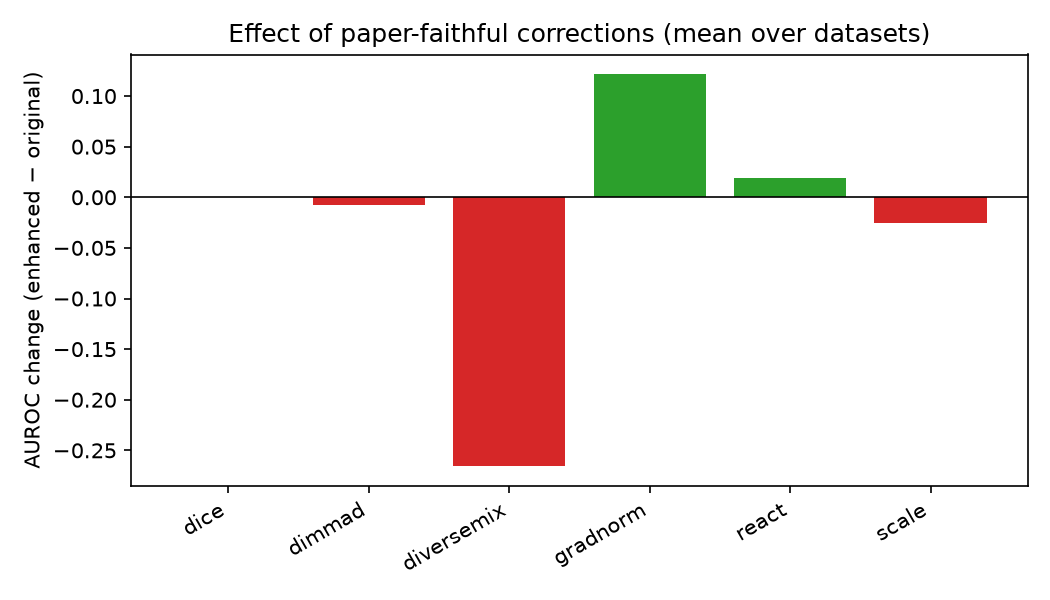
\includegraphics[width=0.85\textwidth]{ablation_delta.png}
\caption{Change in mean AUROC from the original implementation to the paper-faithful
corrected (\texttt{\_enh}) variant, for the six corrected detectors. Positive bars
denote improvement. The gradient-norm repair yields the largest gain ($+0.122$) yet
still lands below chance, while the diversification correction reverses on real data
($-0.266$); no correction lifts a post-hoc detector into competitiveness with the
feature-space methods.}
\label{fig:app_ablation}
\end{figure}

\section{ROC Curves and Score-Distribution Case Study}\label{app:roc}

\begin{figure}[h]
\centering
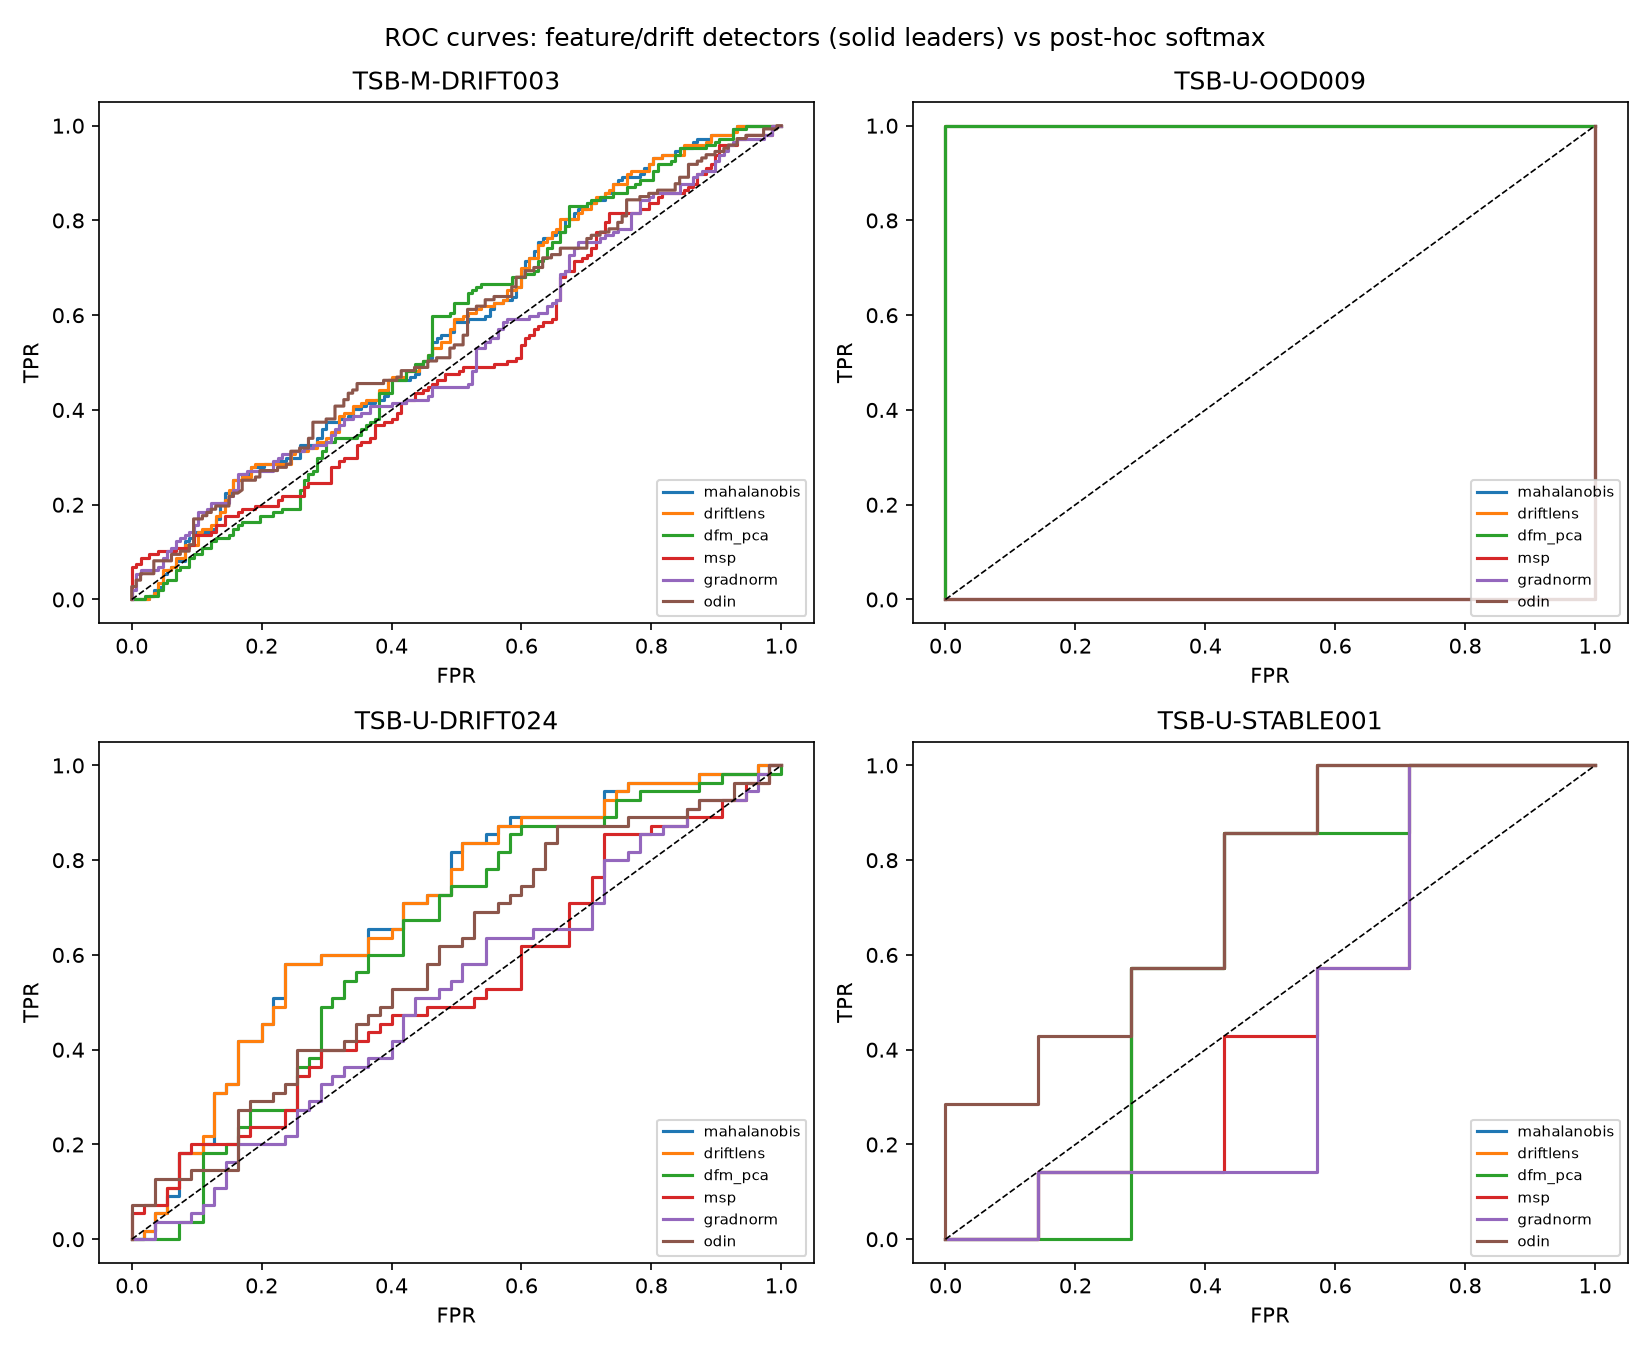
\includegraphics[width=0.95\textwidth]{appendix_roc.png}
\caption{Receiver-operating-characteristic curves for three leading feature/drift
detectors and three post-hoc softmax detectors on a representative
global-normalised dataset. The softmax curves fall below the diagonal, the signature
of score inversion, while the feature-space curves hug the top-left corner.}
\label{fig:app_roc}
\end{figure}

\begin{figure}[h]
\centering
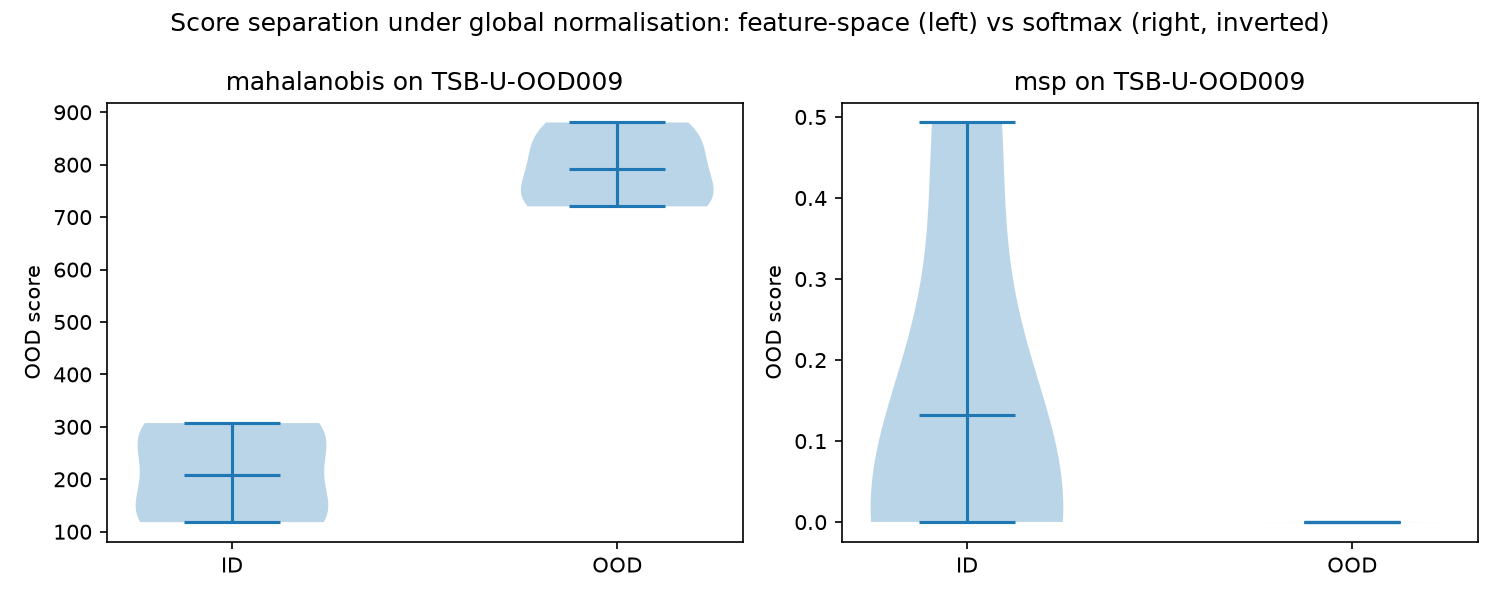
\includegraphics[width=0.9\textwidth]{appendix_violin_case.png}
\caption{Distribution of out-of-distribution scores for in-distribution versus
out-of-distribution test windows on a global-normalised dataset. The feature-space
detector (left) assigns systematically higher scores to OOD windows; the softmax
detector (right) assigns them \emph{lower} scores, inverting the decision and
producing an AUROC below chance --- the mechanism analysed in the main text.}
\label{fig:app_violin}
\end{figure}

\section{Reproducibility}\label{app:repro}

All experiments fix the random seed to \num{42} and run on CPU under Python~3.13 with
PyTorch, NumPy, SciPy, and scikit-learn. The backbone is a 1-D ResNet trained for
\num{40} epochs with cross-entropy over temporal pseudo-classes. The benchmark
comprises \num{36} datasets (\num{18} TSB-StreamingAD-U and \num{18}
TSB-StreamingAD-M, six per DRIFT/OOD/STABLE cell), \num{22} detectors, and \num{772}
completed runs. Per-run configurations and metrics are stored alongside the aggregate
results matrix, and the tables and figures in this manuscript are regenerated
directly from it. The reduced epoch budget and the stratified subsample of \num{36}
of the \num{600} available files are recorded explicitly as scoping decisions; SRS is
excluded on TSB-StreamingAD-M because it hangs on multivariate input, and Outlier
Exposure and DivOE are reported as energy baselines because faithful
auxiliary-outlier training is not available.


\end{document}
